\documentclass[12pt]{amsart}
\usepackage[utf8]{inputenc}


\makeatletter
\def\specialsection{\@startsection{section}{1}%
  \z@{\linespacing\@plus\linespacing}{.5\linespacing}%
%  {\normalfont\centering}}% DELETED
  {\normalfont}}% NEW
\def\section{\@startsection{section}{1}%
  \z@{.7\linespacing\@plus\linespacing}{.5\linespacing}%
%  {\normalfont\scshape\centering}}% DELETED
  {\normalfont\scshape}}% NEW
\makeatother

\makeatletter
\def\@tocline#1#2#3#4#5#6#7{\relax
  \ifnum #1>\c@tocdepth % then omit
  \else
    \par \addpenalty\@secpenalty\addvspace{#2}%
    \begingroup \hyphenpenalty\@M
    \@ifempty{#4}{%
      \@tempdima\csname r@tocindent\number#1\endcsname\relax
    }{%
      \@tempdima#4\relax
    }%
    \parindent\z@ \leftskip#3\relax \advance\leftskip\@tempdima\relax
    \rightskip\@pnumwidth plus4em \parfillskip-\@pnumwidth
    #5\leavevmode\hskip-\@tempdima
      \ifcase #1
       \or\or \hskip 1em \or \hskip 2em \else \hskip 3em \fi%
      #6\nobreak\relax
    \dotfill\hbox to\@pnumwidth{\@tocpagenum{#7}}\par
    \nobreak
    \endgroup
  \fi}
\makeatother
%\usepackage{hyperref}

\addtolength{\hoffset}{-2.25cm}
\addtolength{\textwidth}{4.5cm}
\addtolength{\voffset}{-2.5cm}
\addtolength{\textheight}{5cm}
\setlength{\parskip}{0pt}
\setlength{\parindent}{15pt}

\usepackage{amsmath , amssymb , amsthm}
\makeatletter
\renewcommand*\env@matrix[1][*\c@MaxMatrixCols c]{%
  \hskip -\arraycolsep
  \let\@ifnextchar\new@ifnextchar
  \array{#1}}
\makeatother
\usepackage[colorlinks = true, linkcolor = black, citecolor = black, final]{hyperref}
\usepackage{graphicx}
\usepackage{multicol}
\usepackage{ marvosym }
\usepackage{wasysym}
\usepackage{tikz}
%\usepackage{amsmath}
\usepackage{fancyhdr}
\usepackage{romannum}
\usepackage{mathtools}
\usepackage{listings}
\usepackage{xcolor}
\usepackage{tcolorbox}
\tcbuselibrary{minted,breakable,xparse,skins}
\usepackage{caption}
\usepackage{booktabs}


\definecolor{bg}{gray}{0.95}
\DeclareTCBListing{mintedbox}{O{}m!O{}}{%
  breakable=true,
  listing engine=minted,
  listing only,
  minted language=#2,
  minted style=default,
  minted options={%
    linenos,
    gobble=0,
    breaklines=true,
    breakafter=,,
    fontsize=\small,
    numbersep=8pt,
    #1},
  boxsep=0pt,
  left skip=0pt,
  right skip=0pt,
  left=25pt,
  right=0pt,
  top=3pt,
  bottom=3pt,
  arc=5pt,
  leftrule=0pt,
  rightrule=0pt,
  bottomrule=2pt,
  toprule=2pt,
  colback=bg,
  colframe=white!70,
  enhanced,
  overlay={%
    \begin{tcbclipinterior}
    \fill[gray!20!white] (frame.south west) rectangle ([xshift=20pt]frame.north west);
    \end{tcbclipinterior}},
  #3}
%\usepackage{pythonhighlight}
\usepackage{minted}
\usepackage{biblatex}
\addbibresource{1.bib}

\usemintedstyle{borland}
\usepackage{pythonhighlight}
\usetikzlibrary{patterns}
\newcommand{\ds}{\displaystyle}
\DeclareMathOperator{\sech}{sech}
\setlength{\parindent}{0in}
\pagestyle{plain}

%\pagestyle{empty}
\usemintedstyle{borland}
\newcommand\norm[1]{\left\lVert#1\right\rVert}

\renewcommand{\contentsname}{Table of Contents}




\begin{document}

\begin{titlepage}
   \begin{center}
       \vspace*{1cm}

       \textbf{Computational Neuroscience}

       \vspace{0.7cm}
        \textbf{EEE 482/582}
            
       \vspace{0.7cm}

       \textbf{Can Kocagil} 
       
       \vspace{0.7cm}
       \textbf{21602218}

       %\vfill
       \vspace{0.7cm}
            
       \textbf{Homework-4}
            
       \vspace{0.8cm}
         \begin{figure}[h]
            \centering
            
\includegraphics[width = 0.35\textwidth]{images/bilkent_logo.png}
            %\caption{}
            %\label{fig:mesh1}
        \end{figure}
      % 
\includegraphics[width=0.4\textwidth]{images/bilkent_logo.png}
       \vspace{0.7cm}  
       Department of Electric \& Electronics Engineering \\
       \vspace{0.7cm}
       Bilkent University\\
       \vspace{0.7cm}
       Ankara, Turkey \\
       \vspace{0.7cm}
       25.04.2021
            
   \end{center}
\end{titlepage}

\tableofcontents

\newpage
\listoffigures
\bigskip
\listoftables
%\lstlistoflistings

%\thispagestyle{empty}

\newpage
{\scshape EEE 482} \hfill {\scshape \large  Homework-\romannumeral4\relax} \hfill {\scshape Can Kocagil}
\smallskip
\hrule
\vspace{2mm}

\pagenumbering{arabic}

\section{Question 1}

In this question, stimuli consisting of face images have been used in a study on visual perception and experimental stimuli are provided in the file hw4\_data1.mat, which contains face images down-sampled to a 32 x 32 square grid.

\subsection{Part A}

In part a, the researcher would like to fit encoding models between the stimuli (i.e., face images) and the measured neural responses. To do that, one first needs to define explanatory variables (i.e., regressors) that capture important variations in stimulus properties during the experiments. To accomplish this goal, we will perform Principal Component Analysis (PCA) on face images. Then, we will explore the the captured variance by PCA with different number of principal components.

\bigskip

The curse of dimensionality is a common problem for ML pipelines and refer to various phenomena that arise when analyzing and organizing data in high-dimensional spaces that do not occur in low-dimensional settings \cite{enwiki:1009164221}. Moreover, high dimensional data manifest during analyzing or visualizing the data to identify patterns, and some manifest while training machine learning models. Hence, many ML algorithms are prune to higher dimensional feature spaces so that they are likely to overfit in a statistical sense. Simultaneously, when the researcher would like to fit encoding models between the stimuli and the measured neural responses, the curse of dimensionality is also  neuroscientifically challenged problem. Hence, before encoding the process, eliminating some features or projecting them to lower dimensional space is critical. In this work, we'll work with PCA algorithm to reduce the dimensionality of the face images while trying to keep the information in the original feature space.

\bigskip
PCA is an unsupervised, non-parametric machine learning algorithm primarily used for dimensionality reduction. By PCA, we can extract information from high dimensional features space by projecting it into lower dimensional subspace while preserving the most of the variation in the data. Hence, the aim of the PCA algorithm is to produce principal components (PCs) that are orthogonal in direction that capture the most of the variance in the given data. It is linear algorithm seeks for the greatest variability in the orthogonal (uncorrelated) directions in the subspace. Hence, the underlying assumption in PCA is that data lies on or near a low d-dimensional linear subspace. 

\bigskip
Let's deep dive into PCA. Principal Components (PC) are orthogonal directions that capture most of the variance in the data. For example, 1st PC represent the direction of greatest variability in data. In other means, projection of data points along 1st PC discriminate the data most along any one direction. Let $v_1,...,v_d$ denote the principal directions such that they are orthogonal and unit norm.

\begin{equation}
    v_i^Tv_j = 0 \textit{ and } v_i^Tv_i = 1 \hspace{2mm}  i \neq j  \hspace{2mm} \forall i,j 
\end{equation}

Then, the ultimate aim is to find a vector that maximizes the sample variance of the projections.


\begin{equation}
    \underset{v}{\mathrm{max}} \frac{1}{n} \sum_{i=1}^n (v^Tx_i)^2 = \underset{v}{\mathrm{max}} \hspace{2mm} \textbf{$v^{T}XX^{T}V $} \textit{ s.t. $v^Tv = 1$}
\end{equation}


\newpage
{\scshape EEE 482} \hfill {\scshape \large  Homework-\romannumeral4\relax} \hfill {\scshape Can Kocagil}
\smallskip
\hrule
\vspace{2mm}

Then, the problem becomes constrained optimization problem in the sense of Lagrangian.

\begin{align}
    Lagrangian: \operatorname*{max}_v v^TXX^Tv -\lambda v^Tv
\end{align}
  
 
Hence, $\frac{\partial (v^TXX^Tv -\lambda v^Tv)}{\partial v}$ gives the optimal principal axes by wrapping constraint into the objective function.



\begin{align}
   (XX^T - \lambda I)v = 0 \Leftrightarrow (XX^T)v = \lambda v
\end{align}

Then, the problem becomes eigenvalue problem. In these formulation, v becomes the eigenvectors of sample covariance matrix $XX^T$ assuming the data is centered. Hence, the eigenvalue $\lambda$ denote the amount of variability captured along that dimension. Further, since $\lambda_1 > \lambda_2, > ...$, the first PC captures the greatest variance in the data and it is associated with the largest eigenvalue. Hence, solving the above eqn (4) as a eigenvalue formulation, gives the principal directions so that we can then project our data into computed principal directions. As a another interpretation of PCA, it finds the vectors $v$ such that projections on to the vectors solves the sum of squared, specifically MSE, reconstruction. These reconstructions represents the lower rank estimations of original data space. Finally, once we got principal axes, we project our original data space into these that are called transformed representation projections.


\begin{align}
    \textit{Transformed Representation Projections } = [v_1^Tx_i,...,v_d^Tx_i]
\end{align}


\bigskip
We're ready to apply PCA to face images. In the question settings, we need to perform PCA on 1000 face images with 100PCs. Before that, let's visualize some sample images to explore faces. Here I also put the libraries that I used along that homework.


\begin{mintedbox}{python}
# Imports:
import numpy as np, matplotlib.pyplot as plt, scipy.stats as stats, pandas as pd
from sklearn.decomposition import PCA, FastICA, NMF
import random, h5py

settings = np.seterr(all='ignore')
\end{mintedbox}

Hence, I utilize the \textbf{scikit-learn} library to perform unsupervised algorithms along that homework. Let's visualize some images and their spatial structures.

\begin{mintedbox}{python}
# Retrieving data:
faces = h5py.File('hw4_data1.mat','r')['faces'][:].T

# Little bit of dimension manipulation for representing images:
N, num_pixel = faces.shape
image_faces = faces.reshape(N, np.int(np.sqrt(num_pixel)), np.int(np.sqrt(num_pixel)))
print(image_faces.shape)


# Let's look at the face images:
fig, axs = plt.subplots(3,3,figsize = (8,8))
for i, axes in enumerate(axs.flatten()):
    axes.imshow(image_faces[i], cmap = 'gray')
    axes.axis('off')
\end{mintedbox}



\newpage
{\scshape EEE 482} \hfill {\scshape \large  Homework-\romannumeral4\relax} \hfill {\scshape Can Kocagil}
\smallskip
\hrule
\vspace{2mm}



\begin{figure}[h]
    \centering
        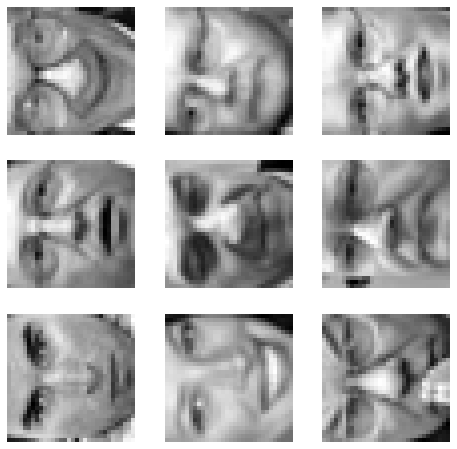
\includegraphics[width = 0.8\textwidth,angle=270,origin=c]{images/Q1/face_images.png}
        \caption{Sample stimuli face images}
    %\label{fig:mesh1}
\end{figure}

As we can see, spatial resolution of stimuli is low as it reduces the computation complexity of the problem. Anyway, let's move on the PCA computation and variance graph w.r.t. PCs.

\begin{mintedbox}{python}
# Latent representation dimension:
latent_dim = 100
pca = PCA(n_components = latent_dim)
principalComponents = pca.fit_transform(faces)

num2str = lambda x : str(round(sum(x),3))

legends = [

    pca.explained_variance_ratio_[:10],
    pca.explained_variance_ratio_[:25],
    pca.explained_variance_ratio_[:50],
    pca.explained_variance_ratio_[:]

]

legends = list(map(num2str,legends))

plt.figure(figsize = (10,5))
plt.plot(pca.explained_variance_ratio_, color = 'r')
plt.xlabel('PCs')
plt.ylabel('Explained Variance')
title = 'Principal Components versus Explained Variance \n'
title += 'First (10,25,50,100) PCs explained variance = '
title += '('  + ' '.join(legends) + ')'
plt.title(title)
plt.grid()
plt.show()

pca_logs = f'Variance explained by PCA for 10 components  {legends[0]} \n'
pca_logs += f'Variance explained by PCA for 25 components  {legends[1]} \n'
pca_logs += f'Variance explained by PCA for 50 components  {legends[2]} \n'
pca_logs += f'Variance explained by PCA for 100 components {legends[3]}'
print(pca_logs)

\end{mintedbox}

\begin{figure}[h]
    \centering
        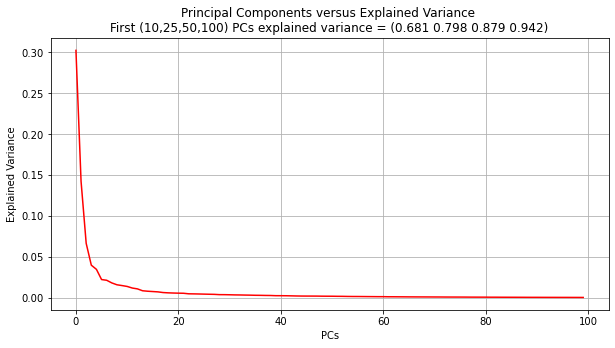
\includegraphics[width = 1\textwidth]{images/Q1/PCA_variance_explained.png}
        \caption{Explained Variance Along PCs}
    %\label{fig:mesh1}
\end{figure}

Variance explained by PCA for 10 components  0.681  \\
Variance explained by PCA for 25 components  0.798  \\
Variance explained by PCA for 50 components  0.879  \\
Variance explained by PCA for 100 components 0.942 \\

As we can see, with the increased number of PCs, we capture greatest number of variance in the data. With just a first 10 PCs, we can explain more than $68\%$ variance in the data. Further, with the first 100PCs, we can almost capture the variance of the original data space as explained more than $94\%$.


\newpage
{\scshape EEE 482} \hfill {\scshape \large  Homework-\romannumeral4\relax} \hfill {\scshape Can Kocagil}
\smallskip
\hrule
\vspace{2mm}

Then, the question asks display the first 25PCs. Let's visualize the first 25PCs as follows.

\begin{mintedbox}{python}
fig, axes = plt.subplots(5, 5, figsize=(12,12))
for i, ax in enumerate(axes.flat):
    ax.imshow(pca.components_[i].reshape(32, 32).T, cmap = 'gray')
    ax.axis('off')
\end{mintedbox}

\begin{figure}[h]
    \centering
        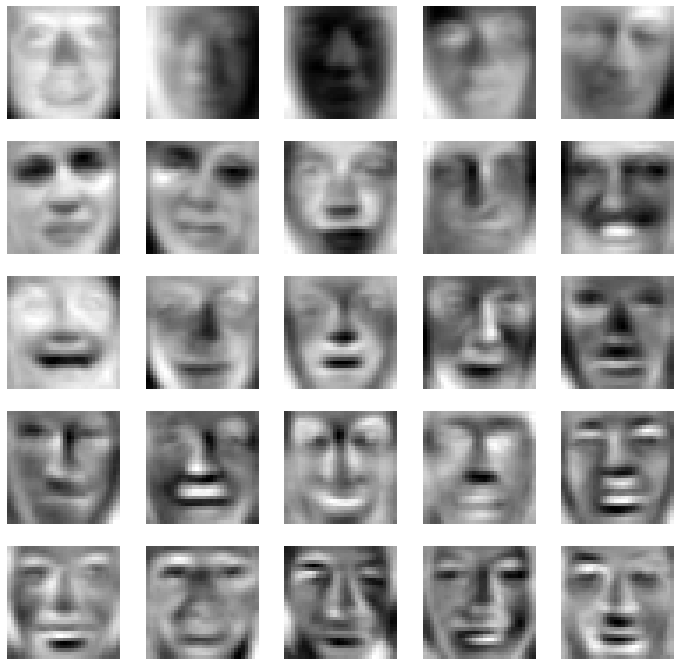
\includegraphics[width = 1\textwidth]{images/Q1/PCA_components_100.png}
        \caption{Visualization of First 25Pcs}
    %\label{fig:mesh1}
\end{figure}

We can see that first 25PCs captures spatial structure of face images with representative facial points such as eyes, nose, eyebrow. Moreover, these are called \textbf{eigen faces} that refer to set of eigenvectors and used in face \& facial recognition applications in the context of computer vision.


\newpage
{\scshape EEE 482} \hfill {\scshape \large  Homework-\romannumeral4\relax} \hfill {\scshape Can Kocagil}
\smallskip
\hrule
\vspace{2mm}

\subsection{Part B}
Then, the researcher would like to know how many PCs are sufficient to obtain a reasonable representation of the stimuli. To explore this, we reconstruct images based on PCs. In other words, we'll estimate the original data space with low rank method based on the computed PCs. Here, the question asks to reconstruct based on first 10, 25, and 50 PCs with their corresponding visualizations. Then, we'll report the error statistics based on MSE loss. Here, I construct 2 utility functions for PCA reconstruction and formatted face plotting as follows.

\begin{mintedbox}{python}
def pca_reconstruction(data:np.ndarray,
                       trained_pca:PCA,
                       number_PCs:int) -> np.ndarray:
    """
        Given the input data, trained PCA variable and # of PCs, reconstruct images based on the PCs components.
            
        Arguments:
            - data (np.ndarray) : Input data
            - trained_pca (PCA) : trained PCA variable
            - number_PCs (int)  : # of PCs to reconstruct images
            
        Returns:
            - reconstructed_data (np.ndarray) : Reconsturcted/Predicted data via given # of PCs
    """
    pca_mean = trained_pca.mean_ 
    mean_removed = data - pca_mean
    pca_components = trained_pca.components_[:number_PCs]
    
    return mean_removed @ pca_components.T @ pca_components + pca_mean

def plot_faces(faces:np.ndarray,
               suptitle:str) -> None:
    """
        Given the face matrix and its suptitle, plots the 6x6 grid of faces.
        
        Arguments:
            - faces       (np.ndarray) : Face data to be plotted
            - suptitle    (str)        : Suptitle of the visualizatiom
            
        Returns:
            - None
    """
    
    fig, axes = plt.subplots(6, 6, 
                             figsize=(10,10),
                             facecolor='white',
                             subplot_kw= {
                                 'xticks': [],
                                 'yticks':[]
                             }
    )
    fig.suptitle(suptitle,
                 fontsize = '14')
                 
    fig.tight_layout(rect = [0, 0, 1, .95])
    
    for i, ax in enumerate(axes.flat):
        ax.imshow(faces[i].reshape(32, 32).T, cmap='gray')
        ax.set_xlabel(i+1)
\end{mintedbox}

Hence, we are ready to reconstruct images based on first 10,25 and 50 PCs.
\begin{mintedbox}{python}
faces_PCA_10 = pca_reconstruction(faces,pca,10)
faces_PCA_25 = pca_reconstruction(faces,pca,25)
faces_PCA_50 = pca_reconstruction(faces,pca,50)
faces_PCA_100 = pca.inverse_transform(principalComponents)
\end{mintedbox}

Note that I also compute the reconstruction of face data based on the 100Pcs to explore the further behavior of estimations. From now on, I visualize the reconstructions and original data space with 36 samples with their corresponding comments. Let's start with the original first 36 faces images.

\begin{mintedbox}{python}
plot_faces(faces,suptitle = 'Original Versions of the First 36 Images')
\end{mintedbox}

\begin{figure}[h]
    \centering
        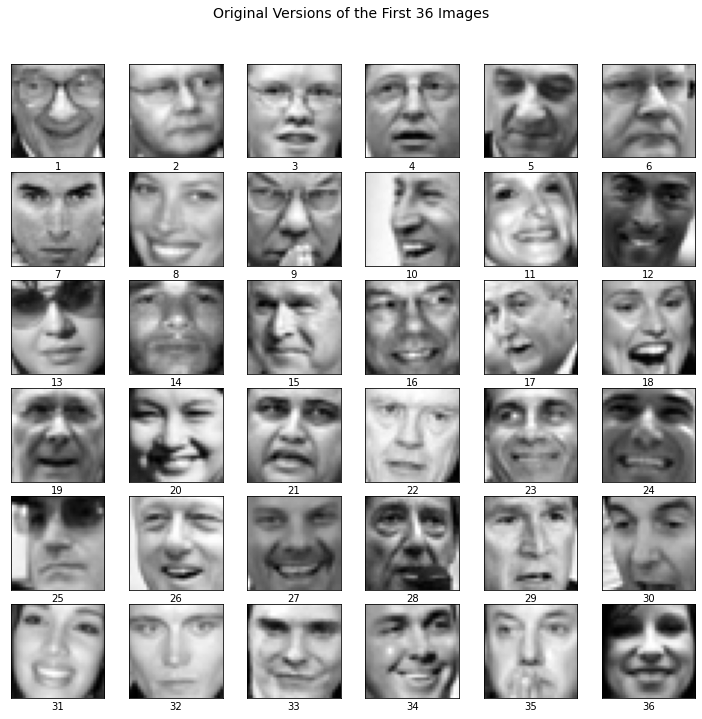
\includegraphics[width = 0.8\textwidth]{images/Q1/Original_face_images_36.png}
        \caption{Visualization of Original First 36 Images}
    %\label{fig:mesh1}
\end{figure}


\newpage
{\scshape EEE 482} \hfill {\scshape \large  Homework-\romannumeral4\relax} \hfill {\scshape Can Kocagil}
\smallskip
\hrule
\vspace{2mm}

\begin{mintedbox}{python}
plot_faces(faces_PCA_10,suptitle = 'Reconstructed 36 images based on first 10 PCs')
\end{mintedbox}

\begin{figure}[h]
    \centering
        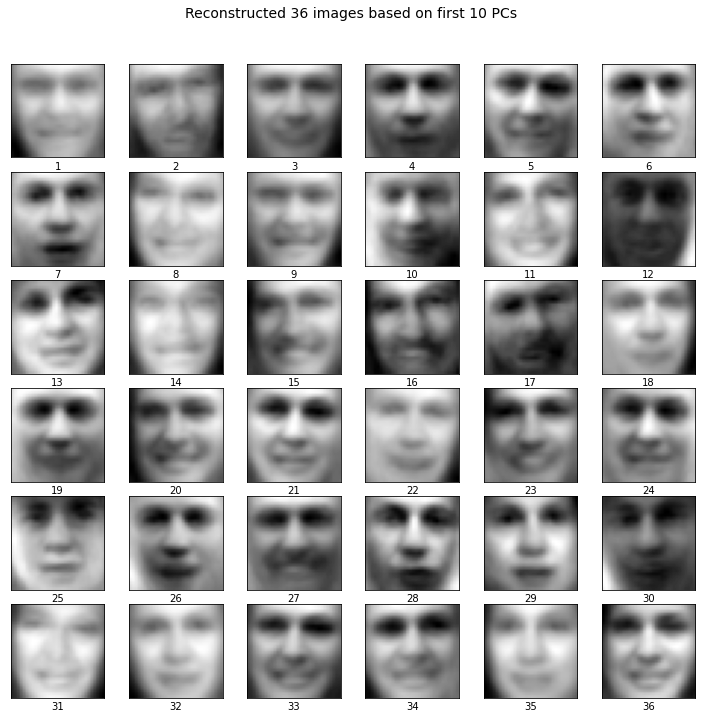
\includegraphics[width = 1\textwidth]{images/Q1/Reconstructed 36 images based on first 10 PCs.png}
        \caption{Reconstructed 36 images based on first 10 PCs}
    %\label{fig:mesh1}
\end{figure}

As we can see, we capture the spatial semantics of the face images just based on the first 10PCs. The reconstructions are quite enough for early experimental purposes.

\newpage
{\scshape EEE 482} \hfill {\scshape \large  Homework-\romannumeral4\relax} \hfill {\scshape Can Kocagil}
\smallskip
\hrule
\vspace{2mm}

\begin{mintedbox}{python}
plot_faces(faces_PCA_25,suptitle = 'Reconstructed 36 images based on first 25 PCs')
\end{mintedbox}

\begin{figure}[h]
    \centering
        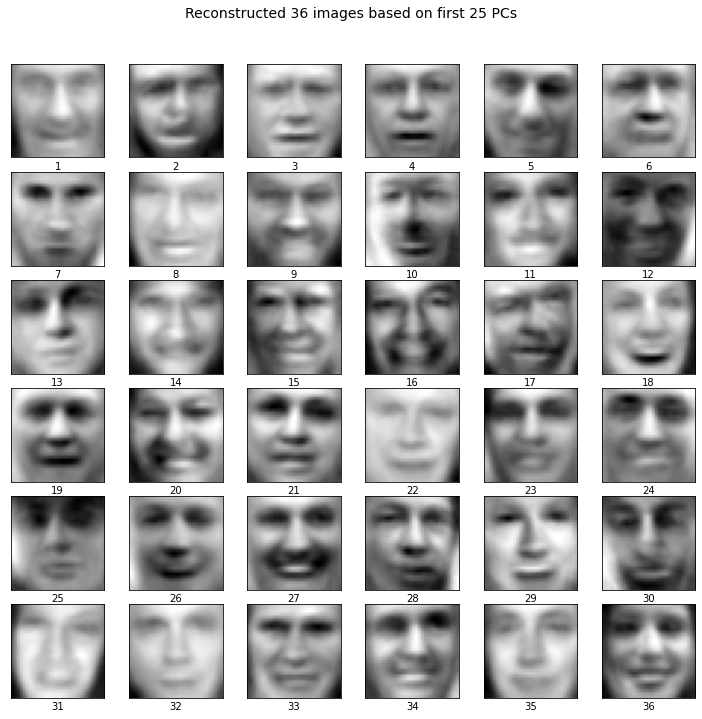
\includegraphics[width = 1\textwidth]{images/Q1/Reconstructed 36 images based on first 25 PCs.png}
        \caption{Reconstructed 36 images based on first 25 PCs}
    %\label{fig:mesh1}
\end{figure}

As we can see, we further capture the spatial semantics of the face images based on the first 25PCs. The facial structures are much more clear, and we see clear distinctions between mutual faces. Probably, facial matching algorithms will match the low rank estimations and original faces accurately. 


\newpage
{\scshape EEE 482} \hfill {\scshape \large  Homework-\romannumeral4\relax} \hfill {\scshape Can Kocagil}
\smallskip
\hrule
\vspace{2mm}

\begin{mintedbox}{python}
plot_faces(faces_PCA_50,suptitle = 'Reconstructed 36 images based on first 50 PCs')
\end{mintedbox}

\begin{figure}[h]
    \centering
        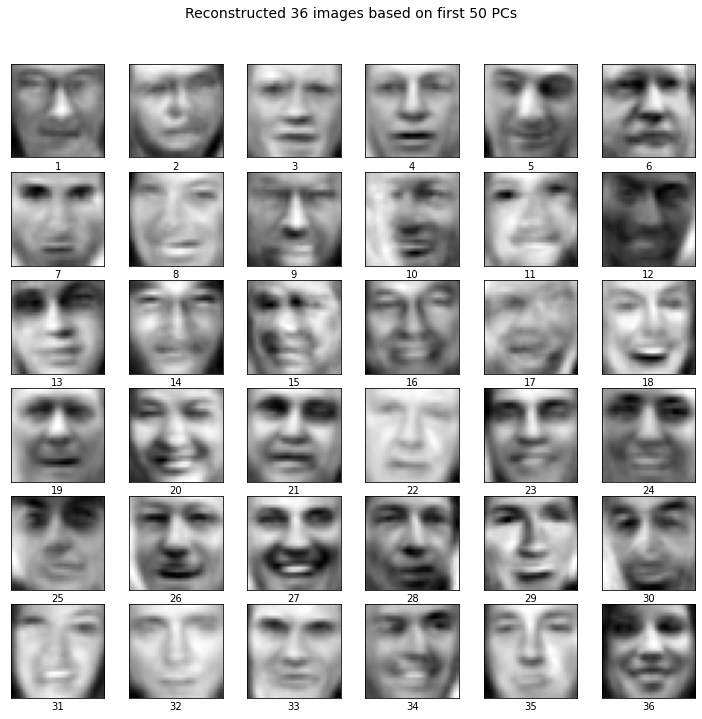
\includegraphics[width = 1\textwidth]{images/Q1/Reconstructed 36 images based on first 50 PCs.png}
        \caption{Reconstructed 36 images based on first 50 PCs}
    %\label{fig:mesh1}
\end{figure}

As we can see, we further capture the high level semantics of the face images based on the first 50PCs. The spatial structure is clear, faces are identifiable by human vision. Moreover, the facial keypoints are much more clear w.r.t. previous reconstructions. Facial landmark detection algorithms can probably start working with these low rank estimations accurately.


\newpage
{\scshape EEE 482} \hfill {\scshape \large  Homework-\romannumeral4\relax} \hfill {\scshape Can Kocagil}
\smallskip
\hrule
\vspace{2mm}

\begin{mintedbox}{python}
plot_faces(faces_PCA_100, suptitle = 'Reconstructed 36 images based on first 100 PCs')
\end{mintedbox}

\begin{figure}[h]
    \centering
        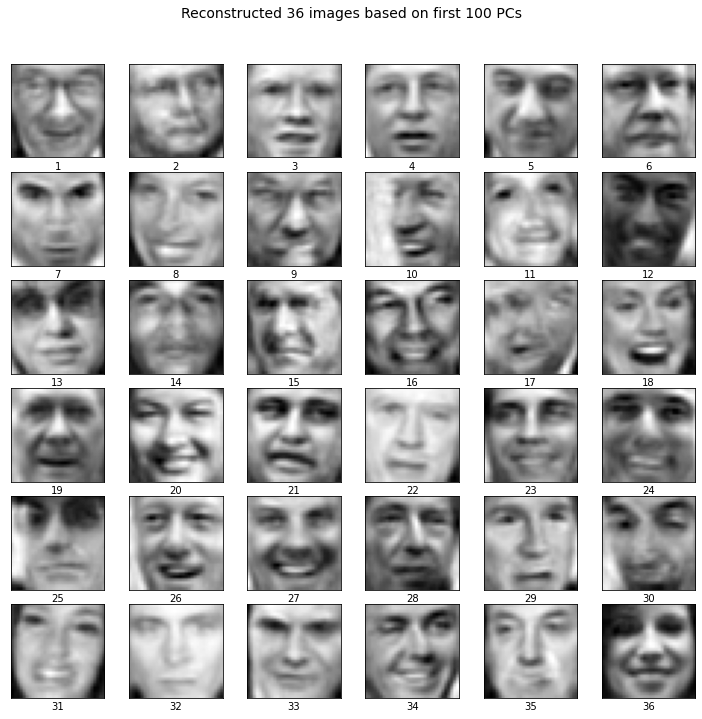
\includegraphics[width = 1\textwidth]{images/Q1/Reconstructed 36 images based on first 100 PCs.png}
        \caption{Reconstructed 36 images based on first 100 PCs}
    %\label{fig:mesh1}
\end{figure}

As we can see, we further capture the semantically meaningful spatial structure of the face images based on the first 100PCs. The reconstructions are quite well as we capture more than $94\%$ of the variability in the original data space.

\newpage
{\scshape EEE 482} \hfill {\scshape \large  Homework-\romannumeral4\relax} \hfill {\scshape Can Kocagil}
\smallskip
\hrule
\vspace{2mm}

Then, let's compute the descriptive statistics of the reconstruction errors based on the MSE loss.

\begin{mintedbox}{python}
def squared_error(y_true:np.ndarray,y_pred:np.ndarray) -> np.ndarray:
    """
        Given the grounth truth matrix and prediction, computes element wise squared error.
        
            
        Arguments:
            - y_true  (np.ndarray) : grounth truth
            - y_pred  (np.ndarray) : prediction
            
        Returns:
            square_error (np.ndarray) : Point-wise MSE loss
    
    """
    assert y_true.shape == y_pred.shape, f'Mismatch Dimension!, {y_true.shape} does not match with {y_pred.shape}'
    return (y_true - y_pred) ** 2
\end{mintedbox}

Then, we compute the average and standard deviation of  MSE loss between original face images and their PCA reconstructions as follows.

\begin{mintedbox}{python}
mse_10 = squared_error(y_true = faces, y_pred = faces_PCA_10)
mse_25 = squared_error(y_true = faces, y_pred = faces_PCA_25)
mse_50 = squared_error(y_true = faces, y_pred = faces_PCA_50)


std_mse_10 = mse_10.mean(-1).std()
std_mse_25 = mse_25.mean(-1).std()
std_mse_50 = mse_50.mean(-1).std()

mean_mse_10 = mse_10.mean()
mean_mse_25 = mse_25.mean()
mean_mse_50 = mse_50.mean()


print(f'PCA reconstruction loss stats based on first 10 PCs, \n (mean,std) = {mean_mse_10,std_mse_10}')
print(f'PCA reconstruction loss stats based on first 25 PCs, \n (mean,std) = {mean_mse_25,std_mse_25}')
print(f'PCA reconstruction loss stats based on first 50 PCs, \n (mean,std) = {mean_mse_50,std_mse_50}')
\end{mintedbox}

PCA reconstruction loss stats based on first 10 PCs,  \\
 (mean,std) = (523.2417453440711, 257.6412003257671)\\
PCA reconstruction loss stats based on first 25 PCs, \\
 (mean,std) = (332.2564923164667, 153.11014543812558)\\
PCA reconstruction loss stats based on first 50 PCs, \\
 (mean,std) = (198.4252027189417, 84.17954418126885)\\

As expected, with the increasing number of PCs used in reconstruction, the error measured between original data space and reconstructions are decreased gradually.


\newpage
{\scshape EEE 482} \hfill {\scshape \large  Homework-\romannumeral4\relax} \hfill {\scshape Can Kocagil}
\smallskip
\hrule
\vspace{2mm}


\subsection{Part C}
In this part the question, instead of PCA, we'll find explanatory variables to capture stimulus properties using independent component analysis (ICA). We'll perform the same analysis with ICA instead of PCA.

\bigskip
Let's discuss the internal structure of ICA algorithm and their use cases. ICA is computational method for separating a multivariate signal into additive subcomponents. This is done by assuming that the subcomponents are non-Gaussian signals and that they are statistically independent from each other \cite{enwiki:1007441084}. These settings are necessary and sufficient for encoding source signals and their mixing properties for ICA. ICA seeks for orthogonal rotation of pre-whitened data with iterative schedule that maximizes the non-Gaussianity of the rotated components \cite{enwiki:1007441084}. Here, non-Gaussianity property is required for finding orthogonal directions and serves as a proxy for independence in the statistical sense. Whitening is required for ICA computations. Whitening is a statistical transformation in such a way that potential correlations between its components are removed (covariance equal to 0) and the variance of each component is equal to 1. Ones the data is whitened, we can perform ICA analysis. 

\bigskip
Let's dive into analytical formulation of ICA. In the Sparse Coding settings, one wanted to learn a latent representation as in the case of neurobiological settings. In ICA, we want to learn linearly represented subspace with strict orthonormality properties. More precisely, given the data $X$, ICA seeks for a set of basis vectors that is represented in the matrix $W$ such that features are sparse and the representation is orthonormal. Hence, with these analytical properties, we can construct objective function $J(W)$ as follows.

\begin{equation}
    J(W) = \norm{WX}_1 \textit{ s.t. } WW^T = I
\end{equation}

Hence, the ICA problem turns the optimization problem as in the all cases of ML pipelines. There are various ways to optimize the objective function but generally there is no simple analytical solution as usually in the case in ML. Moreover, orthonormality property also make the optimization problem harder. For example, $J(W)$ can be optimized with gradient descent based algorithms but the gradient in the direction of convergence must be followed by a step that maps the new basis back to the space of orthonormal bases. It is feasible but generally slow. Also, there are non-iterative methods for computing ICA that are slightly more complicated than iterative settings. However, the main idea is same. Anyway, these are not the concepts of this homework, let's back to our problem.

\bigskip
There are bunch of ICA algorithms with different degree of computational complexities. In these work, we'll work with the FastICA algorithm to find explanatory variables of face images.Here is the code for computation of FastICA with scikit-learn library.


\begin{mintedbox}{python}
fastIca_10 = FastICA(n_components = 10, random_state = 5)
fastIca_components_10 = fastIca_10.fit_transform(faces)
\end{mintedbox}

With these two lines of Python code, we whitened the data and perform FastICA analysis on face images with the dimensionality 10. Let's visualize the ICs as follows.
\begin{mintedbox}{python}
fig, axes = plt.subplots(2, 5, figsize=(10,4))
for i, ax in enumerate(axes.flat):
    ax.imshow(fastIca_10.components_[i].reshape(32, 32).T, cmap = 'gray')
    ax.axis('off')
\end{mintedbox}


\newpage
{\scshape EEE 482} \hfill {\scshape \large  Homework-\romannumeral4\relax} \hfill {\scshape Can Kocagil}
\smallskip
\hrule
\vspace{2mm}

\begin{figure}[h]
    \centering
        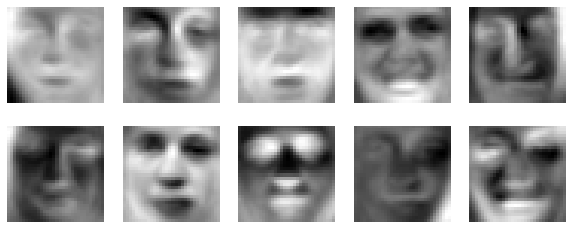
\includegraphics[width=0.7\linewidth,height=0.7\textheight,keepaspectratio]{images/Q1/fastICA_10_components.png}
        \caption{Visualization of 10 ICs}
    %\label{fig:mesh1}
\end{figure}

FastICA algorithm capture the spatial semantics of face images with 10 components. Let's see further visualization of  components with higher degree of ICs as follows.

\begin{mintedbox}{python}
fastIca_25 = FastICA(n_components = 25,whiten = True, random_state = 5)
fastIca_components_25 = fastIca_25.fit_transform(faces)


fig, axes = plt.subplots(5, 5, figsize=(10,10))
for i, ax in enumerate(axes.flat):
    ax.imshow(fastIca_25.components_[i].reshape(32, 32).T, cmap = 'gray')
    ax.axis('off')
\end{mintedbox}

\begin{figure}[h]
    \centering
        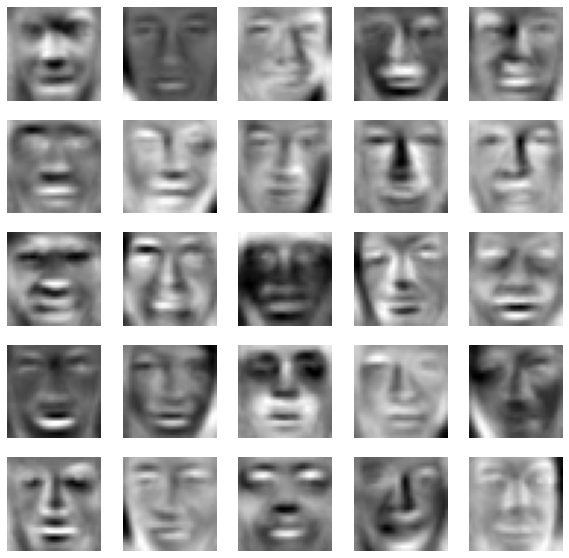
\includegraphics[width = 0.7\textwidth]{images/Q1/fastICA_25_components.png}
        \caption{Visualization of 25 ICs}
    %\label{fig:mesh1}
\end{figure}

\newpage
{\scshape EEE 482} \hfill {\scshape \large  Homework-\romannumeral4\relax} \hfill {\scshape Can Kocagil}
\smallskip
\hrule
\vspace{2mm}

As we can see, with the increasing number of IC components, the spatial structure of face images are much more clear and intuitive. Let's see more with higher number of ICs.


\begin{mintedbox}{python}
fastIca_50 = FastICA(n_components = 50, random_state = 5)
fastIca_components_50 = fastIca_50.fit_transform(faces)


fig, axes = plt.subplots(5, 10, figsize=(20,10))
for i, ax in enumerate(axes.flat):
    ax.imshow(fastIca_50.components_[i].reshape(32, 32).T, cmap = 'gray')
    ax.axis('off')
\end{mintedbox}

\begin{figure}[h]
    \centering
        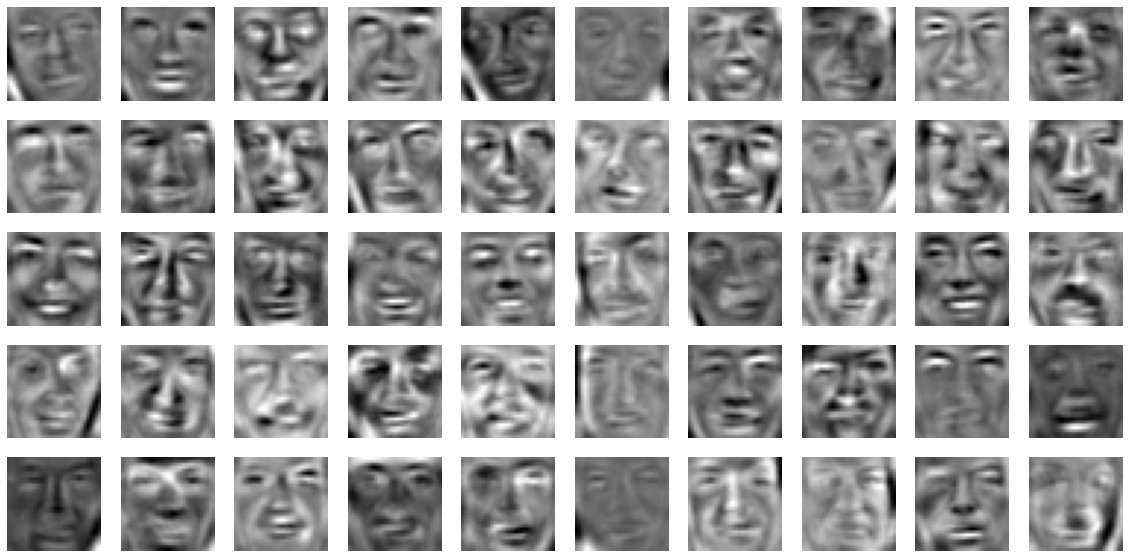
\includegraphics[width = 1\textwidth]{images/Q1/fastICA_50_components.png}
        \caption{Visualization of 50 ICs}
    %\label{fig:mesh1}
\end{figure}

Then, the next part is ICA reconstructions based on the 10,25 and 50 IC components. 

\begin{mintedbox}{python}
faces_ICA_10 = fastIca_10.inverse_transform(fastIca_components_10)
faces_ICA_25 = fastIca_25.inverse_transform(fastIca_components_25)
faces_ICA_50 = fastIca_50.inverse_transform(fastIca_components_50)
\end{mintedbox}

Here, I back to original data space with low rank ICA reconstruction based on 10, 25 and 50 ICs. From now on, I visualize the reconstructions sequentially starting from the next page.


\newpage
{\scshape EEE 482} \hfill {\scshape \large  Homework-\romannumeral4\relax} \hfill {\scshape Can Kocagil}
\smallskip
\hrule
\vspace{2mm}

\begin{mintedbox}{python}
plot_faces(faces_ICA_10, suptitle = 'FastICA reconstruction based on 10 independent components')
\end{mintedbox}

\begin{figure}[h]
    \centering
        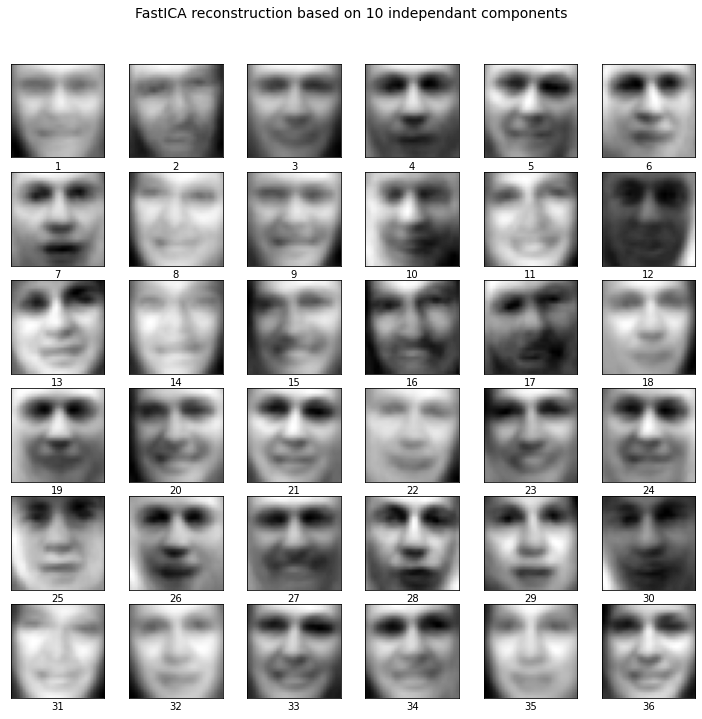
\includegraphics[width = 1\textwidth]{images/Q1/FastICA reconstruction based on 10 independant component.png}
        \caption{FastICA reconstruction based on 10 independent components}
    %\label{fig:mesh1}
\end{figure}

As we can see, we capture the semantically meaningful spatial structure of the face images based on the first 10ICs. The spatial densities are clear to identify by human vision. Further, generalized micro mimics of faces are also come to the fore.    

\newpage
{\scshape EEE 482} \hfill {\scshape \large  Homework-\romannumeral4\relax} \hfill {\scshape Can Kocagil}
\smallskip
\hrule
\vspace{2mm}

\begin{mintedbox}{python}
plot_faces(faces_ICA_25, suptitle = 'FastICA reconstruction based on 25 independent components')
\end{mintedbox}

\begin{figure}[h]
    \centering
        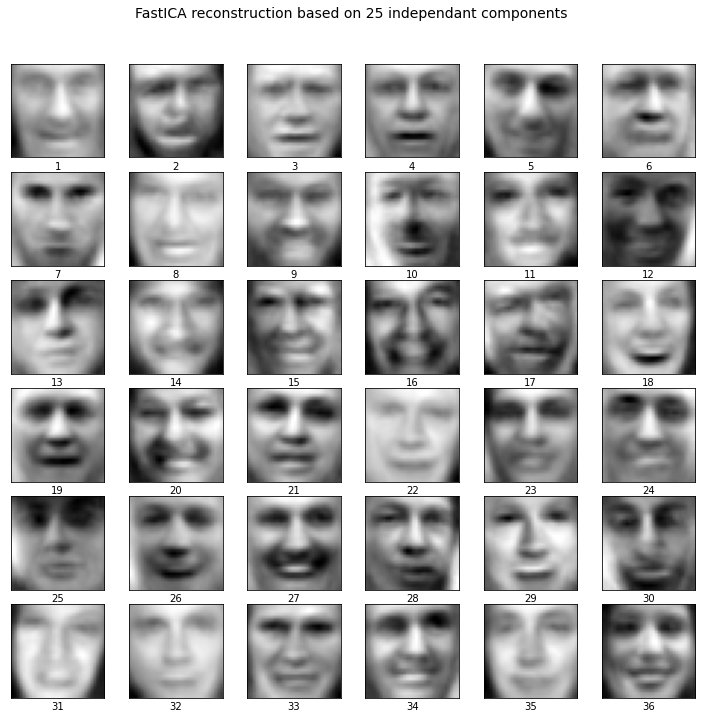
\includegraphics[width = 1\textwidth]{images/Q1/FastICA reconstruction based on 25 independant components.png}
        \caption{FastICA reconstruction based on 25 independent components}
    %\label{fig:mesh1}
\end{figure}


As we can see, we further capture the semantically meaningful spatial structure of the face images based on the first 25 ICs. The spatial densities are much more clear than before. As expected, with increasing dimension of ICA space, we further reason the facial cognitives. 

\newpage
{\scshape EEE 482} \hfill {\scshape \large  Homework-\romannumeral4\relax} \hfill {\scshape Can Kocagil}
\smallskip
\hrule
\vspace{2mm}

\begin{mintedbox}{python}
plot_faces(faces_ICA_50, suptitle = 'FastICA reconstruction based on 50 independent components')
\end{mintedbox}

\begin{figure}[h]
    \centering
        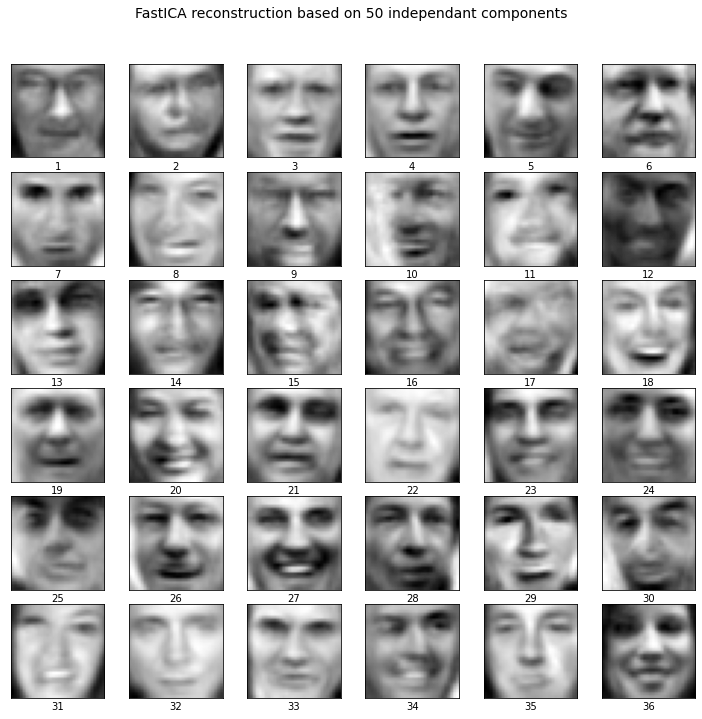
\includegraphics[width = 1\textwidth]{images/Q1/FastICA reconstruction based on 50 independant components.png}
        \caption{FastICA reconstruction based on 50 independent components}
    %\label{fig:mesh1}
\end{figure}

As a last reconstruction, based on 50 ICs, the algorithm captures the greatest semantic in original feature dimensionality as it can be seen from the spatial similarity between face images and its reconstructions.


\newpage
{\scshape EEE 482} \hfill {\scshape \large  Homework-\romannumeral4\relax} \hfill {\scshape Can Kocagil}
\smallskip
\hrule
\vspace{2mm}

Then, let's reason the reconstructions mathematically based MSE loss and its descriptive statistics.

\begin{mintedbox}{python}
mse_10 = squared_error(y_true = faces, y_pred = faces_ICA_10)
mse_25 = squared_error(y_true = faces, y_pred = faces_ICA_25)
mse_50 = squared_error(y_true = faces, y_pred = faces_ICA_50)


std_mse_10 = mse_10.mean(-1).std()
std_mse_25 = mse_25.mean(-1).std()
std_mse_50 = mse_50.mean(-1).std()

mean_mse_10 = mse_10.mean()
mean_mse_25 = mse_25.mean()
mean_mse_50 = mse_50.mean()


print(f'ICA reconstruction loss stats based on first 10 ICs, \n (mean,std) = {mean_mse_10,std_mse_10}')
print(f'ICA reconstruction loss stats based on first 25 ICs, \n (mean,std) = {mean_mse_25,std_mse_25}')
print(f'ICA reconstruction loss stats based on first 50 ICs, \n (mean,std) = {mean_mse_50,std_mse_50}')
\end{mintedbox}

ICA reconstruction loss stats based on first 10 ICs,  \\
 (mean,std) = (523.2417453440557, 257.6412004632383)\\
ICA reconstruction loss stats based on first 25 ICs, \\
 (mean,std) = (332.2564920665104, 153.11028826729745)\\
ICA reconstruction loss stats based on first 50 ICs, \\
 (mean,std) = (198.42506719787565, 84.17996584442903)\\

First things first, FastICA algorithm is internally structured as whitening and orthogonal rotation as rotation yields the greatest non-Gaussianity with rotated direction. Since the whitening process can be accomplished by classical PCA and orthogonal rotation does not affect the reconstruction MSE loss of the ICA, the MSE loss statistics are identical.

\subsection{Part D}
In this section, we'll perform explanatory face image analysis with Non-Negative Matrix Factorization (NNMF) instead of PCA or ICA. The computational procedures are identical except for the dimensionality reduction algorithm as the previous sections. In other words, we'll perform NNMF analysis based on 10, 25 and 50 MFs. We'll perform comprehensive visualizations of MFs with their reconstructions to the original data space. Finally, we'll report error statistics with comparisons to other sections. As usual, let's start with the discussion of the algorithm and its use cases.

\bigskip
NNMF is an unsupervised machine learning algorithm and widely used tool to analyze high dimensional datasets as in the case of PCA and ICA except for non-negativity condition as prior. It extract sparse and meaningful insights from high dimensional non-negative features spaces. It approximates a non-negative low rank data matrix such that $X\approx WH$. Hence, given the data matrix $X_{mxn}$ where the entries of $A$ is stricly non-negative, NNMF learns the $W_{mxk}$ and $W_{kxn}$ such that it gives the estimation of $A$, i.e., $X \approx WH $ where the quantity $k$ is set by the researcher as it denotes the latent dimensionality of the original feature space. Note that $W$ and $H$ are generally called dictionary (or basis) and expansion (or coefficient) matrix, respectively.


\newpage
{\scshape EEE 482} \hfill {\scshape \large  Homework-\romannumeral4\relax} \hfill {\scshape Can Kocagil}
\smallskip
\hrule
\vspace{2mm}

Then, let's formulate the NNMF problem as iterative optimization problem as follows.

\begin{equation}
    \operatorname*{min}_{W \in \mathbb{R}^{mxk},H \in \mathbb{R}^{kxn}} \norm{X-WH}_F^2 \textit{ s.t. } W_{i,j} \geq 0 \textit{ and } H_{j,k} \geq 0  \textit{ } \forall i,j,k
\end{equation}

where $F$ denotes Frobenius norm that gives the intuition that there are Gaussian noise. Note that another norms can be used depending on the application. (Kullback-Leibler divergence for text-mining, the Itakura-Saito distance for music analysis, or the $l_1$ norm to improve robustness against outliers).

\bigskip
Furthermore, NNMF learning is a subclass of NP-hard theoretically, but there are heuristic approximations methods works well in practise. So, the the parameters of NNMF, $W$ and $H$ are not unique. Here, one well-known update rule for $W$ and $H$ as it converges to local minima in the error surface is presented.

\begin{equation}
  H_{\alpha u}  \longleftarrow H_{\alpha u} \sum_{i} W_{i \alpha} \frac{X_{iu}}{(WH)_{iu}} \textit{ and }
  W_{i \alpha}  \longleftarrow W_{i \alpha} \sum_{u} H_{\alpha u } \frac{X_{iu}}{(WH)_{iu}}
\end{equation}

The iteration number is also set by the user before hand. As a final note, as PCA is not localized, oriented to spatial structure of images, NNMF learns a parts-based representation of faces whereas PCA learn holistic representations of images.

\bigskip
Let's move into our case. I set the iteration number as 500 as I observe that this number is a sufficient trade of between accuracy of estimation and its computational complexity. Let's see the code for computation of NNMF and its first 10 components visualization. Note that I also add the absolute value of the minimum of the faces images to shift pixel intensities to positive spatial axis.

\begin{mintedbox}{python}
max_iter = 500
faces += np.abs(np.min(faces))
NMF_10 = NMF(n_components = 10, max_iter = max_iter)
NMF_components_10 = NMF_10.fit_transform(faces)


fig, axes = plt.subplots(2, 5, figsize=(10,4))
for i, ax in enumerate(axes.flat):
    ax.imshow(NMF_10.components_[i].reshape(32, 32).T, cmap = 'gray')
    ax.axis('off')
\end{mintedbox}

\begin{figure}[h]
    \centering
        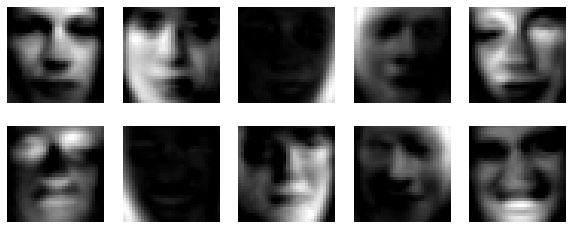
\includegraphics[width = 0.8\textwidth]{images/Q1/NMF_10_components.png}
        \caption{Visualization of NNMF 10 MFs}
    %\label{fig:mesh1}
\end{figure}


\newpage
{\scshape EEE 482} \hfill {\scshape \large  Homework-\romannumeral4\relax} \hfill {\scshape Can Kocagil}
\smallskip
\hrule
\vspace{2mm}

Let's also visualize the further MFs as follows.

\begin{mintedbox}{python}
NMF_25 = NMF(n_components = 25, max_iter = max_iter)
NMF_components_25 = NMF_25.fit_transform(faces)


fig, axes = plt.subplots(5, 5, figsize=(10,10))
for i, ax in enumerate(axes.flat):
    ax.imshow(NMF_25.components_[i].reshape(32, 32).T, cmap = 'gray')
    ax.axis('off')
\end{mintedbox}

\begin{figure}[h]
    \centering
        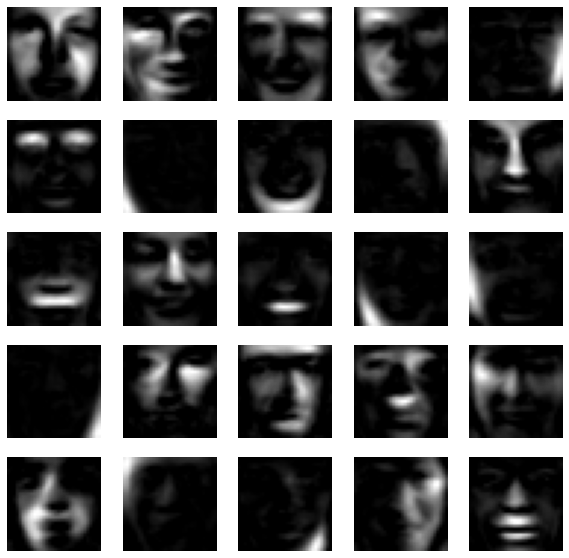
\includegraphics[width = 0.8\textwidth]{images/Q1/NMF_25_components.png}
        \caption{Visualization of NNMF 25 MFs}
    %\label{fig:mesh1}
\end{figure}


\newpage
{\scshape EEE 482} \hfill {\scshape \large  Homework-\romannumeral4\relax} \hfill {\scshape Can Kocagil}
\smallskip
\hrule
\vspace{2mm}

\begin{mintedbox}{python}
NMF_50 = NMF(n_components = 50, max_iter = max_iter)
NMF_components_50 = NMF_50.fit_transform(faces)


fig, axes = plt.subplots(5, 10, figsize=(12,6))
for i, ax in enumerate(axes.flat):
    ax.imshow(NMF_50.components_[i].reshape(32, 32).T, cmap = 'gray')
    ax.axis('off')
\end{mintedbox}

\begin{figure}[h]
    \centering
        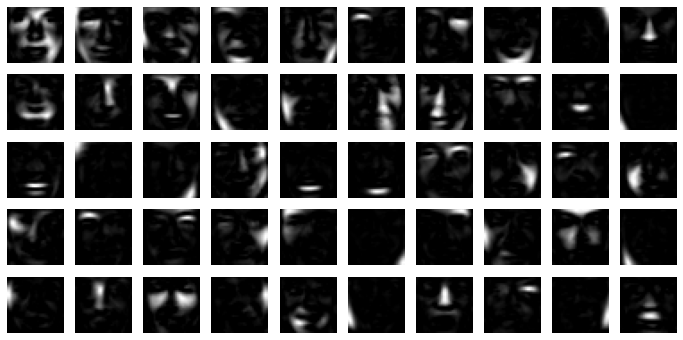
\includegraphics[width = 1\textwidth]{images/Q1/NMF_50_components.png}
        \caption{Visualization of NNMF 50 MFs}
    %\label{fig:mesh1}
\end{figure}


As we can see, with the increasing number of MFs, we capture different spatial information regarding the face images. Some of the components focused on the orientations, while others focused on  facial keypoints, face structures etc.

\bigskip
Let's move on the reconstructions based on 10, 25, and 50 MFs with their correspoding MSE loss statistics as follows.

\begin{mintedbox}{python}
faces = h5py.File('hw4_data1.mat','r')['faces'][:].T
faces_NNMF_10 = NMF_10.inverse_transform(NMF_components_10) - np.abs(np.min(faces))
faces_NNMF_25 = NMF_25.inverse_transform(NMF_components_25) - np.abs(np.min(faces))
faces_NNMF_50 = NMF_50.inverse_transform(NMF_components_50) - np.abs(np.min(faces))

\end{mintedbox}

Note that the absolute value of the minimum of the faces are subtracted from the reconstructions since we added these terms as we are preparing faces images to the NNMF algorithm. Also note that, since I did not use another variable for added version of face images, I read the face image data again, then subtract the the absolute value of the minimum values of the face image data data. 

\newpage
{\scshape EEE 482} \hfill {\scshape \large  Homework-\romannumeral4\relax} \hfill {\scshape Can Kocagil}
\smallskip
\hrule
\vspace{2mm}

\begin{mintedbox}{python}
plot_faces(faces_NNMF_10, suptitle = 'NNMF Reconstruction of faces based on 10MFs')
\end{mintedbox}

\begin{figure}[h]
    \centering
        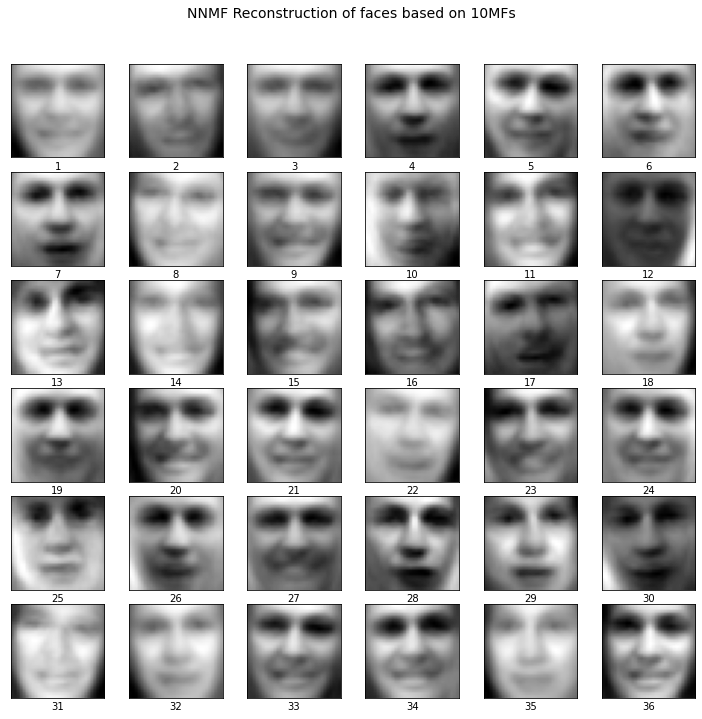
\includegraphics[width = 1\textwidth]{images/Q1/NNMF Reconstruction of faces based on 10MFs.png}
        \caption{NNMF Reconstruction of faces based on 10 MFs}
    %\label{fig:mesh1}
\end{figure}

\newpage
{\scshape EEE 482} \hfill {\scshape \large  Homework-\romannumeral4\relax} \hfill {\scshape Can Kocagil}
\smallskip
\hrule
\vspace{2mm}

\begin{mintedbox}{python}
plot_faces(faces_NNMF_25, suptitle = 'NNMF Reconstruction of faces based on 25MFs')
\end{mintedbox}

\begin{figure}[h]
    \centering
        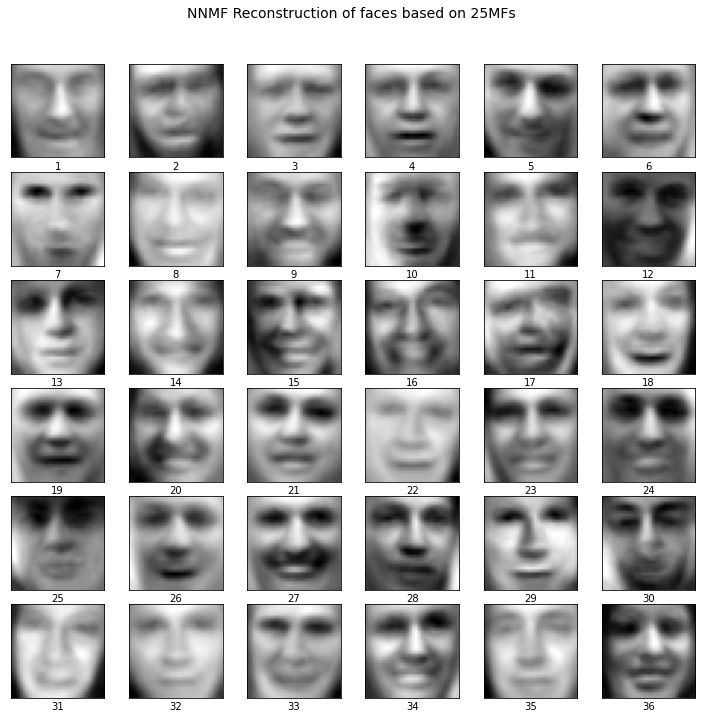
\includegraphics[width = 1\textwidth]{images/Q1/NNMF Reconstruction of faces based on 25MFs.png}
        \caption{NNMF Reconstruction of faces based on 25 MFs}
    %\label{fig:mesh1}
\end{figure}


\newpage
{\scshape EEE 482} \hfill {\scshape \large  Homework-\romannumeral4\relax} \hfill {\scshape Can Kocagil}
\smallskip
\hrule
\vspace{2mm}

\begin{mintedbox}{python}
plot_faces(faces_NNMF_50, suptitle = 'NNMF Reconstruction of faces based on 50MFs')
\end{mintedbox}

\begin{figure}[h]
    \centering
        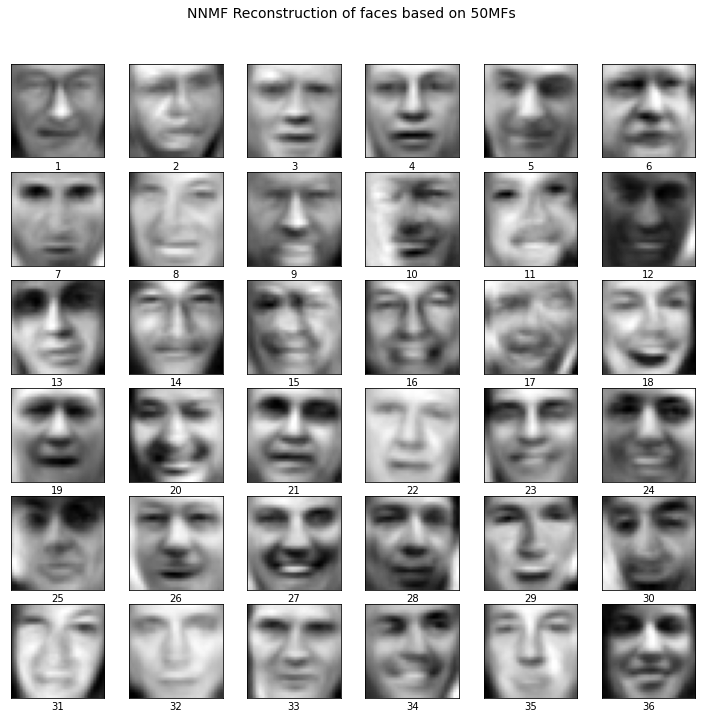
\includegraphics[width = 1\textwidth]{images/Q1/NNMF Reconstruction of faces based on 50MFs.png}
        \caption{NNMF Reconstruction of faces based on 50MFs}
    %\label{fig:mesh1}
\end{figure}

% Buraya birseyler ekle

\newpage
{\scshape EEE 482} \hfill {\scshape \large  Homework-\romannumeral4\relax} \hfill {\scshape Can Kocagil}
\smallskip
\hrule
\vspace{2mm}


Then, let's evaluate our NNMF model based on MSE loss statistics as follows.

\begin{mintedbox}{python}
mse_10 = squared_error(y_true = faces, y_pred = faces_NNMF_10)
mse_25 = squared_error(y_true = faces, y_pred = faces_NNMF_25)
mse_50 = squared_error(y_true = faces, y_pred = faces_NNMF_50)


std_mse_10 = mse_10.mean(-1).std()
std_mse_25 = mse_25.mean(-1).std()
std_mse_50 = mse_50.mean(-1).std()

mean_mse_10 = mse_10.mean()
mean_mse_25 = mse_25.mean()
mean_mse_50 = mse_50.mean()


print(f'NNMF reconstruction loss stats based on first 10 MFs, \n (mean,std) = {mean_mse_10,std_mse_10}')
print(f'NNMF reconstruction loss stats based on first 25 MFs, \n (mean,std) = {mean_mse_25,std_mse_25}')
print(f'NNMF reconstruction loss stats based on first 50 MFs, \n (mean,std) = {mean_mse_50,std_mse_50}')
\end{mintedbox}

NNMF reconstruction loss stats based on first 10 MFs,  \\
 (mean,std) = (533.7720128448966, 267.388838812122)  \\
NNMF reconstruction loss stats based on first 25 MFs,   \\
 (mean,std) = (351.018592518666, 169.342734092105)  \\
NNMF reconstruction loss stats based on first 50 MFs,   \\
 (mean,std) = (221.34231024320826, 103.62372565762264)  \\

We observe that NNMF reconstruction gives the least performance among other methods. The reconstruction statistics are not much different from the ICA and PCA case, but they were slightly better than NNMF. Let's interpret the results and make a discussion.

\bigskip

PCA model produces a new data features as result of combination of existing one while NNMF just decompose a dataset matrix into its non-negative sub matrix whose dimensionality is uneven. Hence, the output of NNMF can be visualized as compressed version of original dataset while reconstructions of PCA uncover the embedding gradients of the spatial data as we previously see. Hence, NNMF outputs are interpretable. In the settings of PCA, we assume that the data lies in lower linear subspace of the original data space. So, non-linear modifications are necessary for the data by nature while NNMF don't require any modifications irrespective of linear separability. Finally, NNMF is sensitive to initialization, hence produces non-unique outputs in every fit while PCA gives the same PCs with different number of trials. According to the error statistics found based on different unsupervised dimension reduction algorithm, PCA and ICA gives the least MSE error hence performed better among others.



\newpage
{\scshape EEE 482} \hfill {\scshape \large  Homework-\romannumeral4\relax} \hfill {\scshape Can Kocagil}
\smallskip
\hrule
\vspace{2mm}


\section{Question 2}
In this question, we consider a population of 21 independent neurons with Gaussian-shaped tuning curves:

\begin{align}
    f_i (x) = A * e^{ - \frac{(x - \mu_i)^2}{2 \sigma ^ 2}}
\end{align}

The tuning curves have an amplitude of 1 and a standard deviation of $\sigma_i$ = 1, with centers
$\mu_i$ evenly spaced between -10 and 10 along the x-axis.

\subsection{Part A}
In this part, we'll plot all tuning curves in the population on the same axis. Then, we'll simulate the  population response to the stimulus $x = -1$ , and plot the population response as a function each neuron's preferred stimulus value.

\bigskip
Let's dive into action. Here I created a Gauss tuning function that produce Gaussian shaped tuning function of a population of neurons as follows.

\begin{mintedbox}{python}
def gauss_tuning(x:np.ndarray = np.linspace(-15, 16, 500),
                 mu:float = 1,
                 sigma:float = 1,
                 A:float = 1) -> np.float16:
    """
        Gaussian shaped tuning function of a population of neurons.

        Arguments:
            x     (np.ndarray)   : The input stimulus parameters
            A     (float)        : Gain of the Gaussian-shaped tuning curve
            mu    (float)   : Mean of the Gausssian-shaped tuning curve
            sigma (float)        : Standard deviation of the Gaussian-shaped tuning curve

        Returns:
            response : Resulting neural response
        """             
    return A * np.exp(-0.5 * ((x- mu)/sigma) ** 2)
\end{mintedbox}

Then, I plot the responses as well as their averaged version (as additional) according to hyperparameters given in the question.

\begin{mintedbox}{python}
neural_responses = []
legends = []
stimuli = np.linspace(-15, 16, 500)
means = np.arange(-10, 11)
plt.figure(figsize=(10,5))

for mean in means:
    response = gauss_tuning(mu = mean)
    plt.plot(stimuli, response)
    legends.append(f" Response with mean {mean}")
    
    # Let's keep neural responses for future use:
    neural_responses.append(response)

# Plot the tuning profiles
plt.plot(stimuli, np.mean(neural_responses, axis=0), color = '0')
legends.append(f" Average Response")
plt.legend(legends, loc="right", bbox_to_anchor=(1.4, 0.5))
plt.xlabel('Stimulus')
plt.ylabel('Activity')
plt.title('Tuning Curves of a Population of Neurons')
plt.grid()
plt.show()
\end{mintedbox}



\begin{figure}[h]
    \centering
        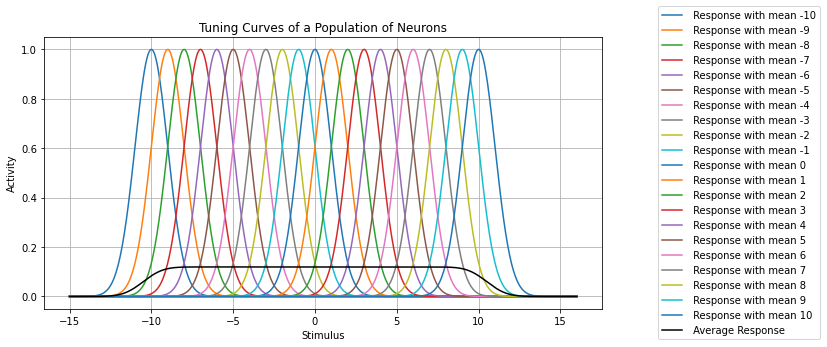
\includegraphics[width = 1\textwidth]{images/Q2/tuning_curves.png}
        \caption{Gaussian Tuning Curves of a Population of Neurons}
    %\label{fig:mesh1}
\end{figure}

As we can see, originated from the Gaussian, each neurons preferred stimulus is the mean of its Gaussian curve. Then, let's see the simulation of the population response to the stimulus with $x = -1$ as follows.


\begin{mintedbox}{python}
kwargs = dict(
            color = '0',
            marker= 'o',
            markerfacecolor='red'
)
plt.figure(figsize=(10,5))
plt.plot(means, gauss_tuning(-1, mu = means),**kwargs)
plt.xlabel('Preferred Stimulus')
plt.ylabel('Population Response')
plt.title('Population Response to the Stimulus x = -1 vs Preferred Stimuli of Neurons')
plt.grid()
plt.show()
\end{mintedbox}

\newpage
{\scshape EEE 482} \hfill {\scshape \large  Homework-\romannumeral4\relax} \hfill {\scshape Can Kocagil}
\smallskip
\hrule
\vspace{2mm}

\begin{figure}[h]
    \centering
        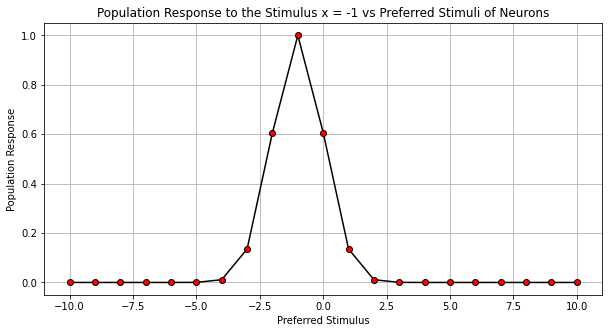
\includegraphics[width = 1\textwidth]{images/Q2/preferred_stimulis.png}
        \caption{Neural Population Response to the Stimulus $x = -1$}
    %\label{fig:mesh1}
\end{figure}

As we distributed the neural responses as a Gaussian, preferred stimulus is where the stimulus that elicits a maximal response. It is expected due to the Gaussian properties.

\subsection{Part B}
In this part of the question, we'll perform a simulated experiment with 200 trials, in each trial we sample a stimulus intensity uniformly from the interval $[-5,5]$ simulate the 21-long vector of population response. Also, we assume the corruption of neural response described by the centered Gaussian noise with $\sigma /20$. Then, the next is to decode the neural response by the Winter-Take-All decoder. Winner-take-all is a computational principle applied in computational models of neural networks by which neurons in a layer compete with each other for activation \cite{enwiki:913093990}. In the classical form, only the neuron with the highest activation stays active while all other neurons shut down; however, other variations allow more than one neuron to be active, for example the soft winner take-all, by which a power function is applied to the neurons \cite{enwiki:913093990}. Hence, we'll simply try to find a stimulus that elicits a maximal response among all neural responses. From the computational perspective, the problem is argument maximizer problem as follows.

\begin{equation}
    x_{WTA} = \underset{u_i}{\mathrm{argmax}} \hspace{1mm} r_i
\end{equation}

where  $x_{WTA}$ is the stimulus that maximizes the response (as mean in the Gaussian case) and $r_i$ is the $i^{th}$ neural response. Let's see in action.

\newpage
{\scshape EEE 482} \hfill {\scshape \large  Homework-\romannumeral4\relax} \hfill {\scshape Can Kocagil}
\smallskip
\hrule
\vspace{2mm}

\begin{mintedbox}{python}
def WTA_decoder(stimuli:np.ndarray,response:np.ndarray) -> np.float16:
    """
    Given a population response and  stimuli of the
    neurons, compute the winner-take-all decoder that 
    estimates the actual stimulus as the preferred
    stimulus of the neuron with maximum response

        Arguments:
            stimuli  (np.ndarray): The preferred stimuli of the neurons
            response (np.ndarray): The neural responses
        Returns:
            stimulus (np.float16): the estimated input stimulus that maximizes the response
    """

    response += np.random.normal(loc = 0, scale = 1/20, size = (21,)) 
    return stimuli[np.argmax(response)]
\end{mintedbox}

As we can see, it is simply argument maximizer operation that finds a stimulates that elicits a maximal neural response. Let's see visualization of the performance of WTA decoder with error statistics as follows.

\begin{mintedbox}{python}
n_trials = 200
stimuli_interval = np.linspace(-5,5, 500).tolist()

# To keep 'responses','stimuli','WTA_stimuli','Errors'
stimuli_response_ = []

for stimuli in random.sample(stimuli_interval, n_trials):
    response = gauss_tuning(stimuli, mu = means)
    WTA_stimuli = WTA_decoder(means, response)
    stimuli_response_.append((response, stimuli, WTA_stimuli, np.abs(WTA_stimuli - stimuli)))
 
# Tuples are gathered:
stimuli_response = list(zip(*stimuli_response_))
\end{mintedbox}

Then, here is the visualization.

\begin{mintedbox}{python}
fig = plt.figure(figsize=(10,5))
error = np.array(stimuli_response[-1])
fig.suptitle(f'Error Stats: (mean,std) = {round(error.mean(),2),round(error.std(),2)}')
plt.scatter(range(n_trials), stimuli_response[1], marker="o", color="r", s=30, linewidths=1)
plt.scatter(range(n_trials), stimuli_response[2], marker="x", color="green", s=30, linewidths=1)
plt.xlabel('# of Trials')
plt.ylabel('Stimulus')
plt.title('Actual and WTA Estimated Stimuli Across Trials')
plt.legend(['Actual', 'WTA Estimated'], loc='upper right')
plt.show()
\end{mintedbox}


\newpage
{\scshape EEE 482} \hfill {\scshape \large  Homework-\romannumeral4\relax} \hfill {\scshape Can Kocagil}
\smallskip
\hrule
\vspace{2mm}

\begin{figure}[h]
    \centering
        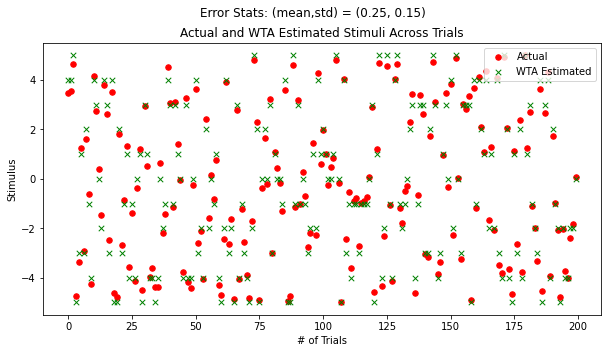
\includegraphics[width = 1\textwidth]{images/Q2/WTA.png}
        \caption{Actual and WTA Estimated Stimuli Across Trials}
    %\label{fig:mesh1}
\end{figure}

As we can see, WTA stimulus shots are not bad, we are closer to actual stimulus. Let's see the error statistics for future comparison.

\begin{mintedbox}{python}
print('Error Statistics for Winner Take All Decoder')
print('Mean of errors in stimuli estimation:', error.mean().round(5))
print('Standard deviation of errors in stimuli estimation :', error.std().round(5))
\end{mintedbox}

Error Statistics for Winner Take All Decoder \\
Mean of errors in stimuli estimation: 0.26058\\
Standard deviation of errors in stimuli estimation : 0.15047\\

Let's move to other decoding algorihtms and then compare our results with WTA decoder.


\subsection{Part C}
In this part, for the same experimental trials simulated in part b, we'll implement a maximum-likelihood decoder, and calculate the stimulus estimate $x_{ML}$ for each trial. As we did in part b, we'll provide estimation error statistics with corresponding visualizations. Let's derive the analytical parts, and apply the trick of logarithmic differentiation to decode neural responses.

\bigskip
Let $x_{ML}$ estimation of the stimulus by MLE algorithm, $r_i$ is the $i^{th}$ response for $i = 1,...21$ that represents the 21 neurons responses. Then, ML decoder try to find a $x_{ML}$ as follows.

\begin{equation}
x_{ML} =  \underset{x}{\mathrm{argmax}} \hspace{1mm} P(r_1,...,r_{21}\mid x)
\end{equation}


The responses of neural population $r_1,...,r_{21}$ is modeled as follows.



\begin{equation}
    r_1,...,r_{21} =  f_{i = 1,...21} (x) + \mathcal{N}(0,(\sigma / 20)^2)
\end{equation}


\newpage
{\scshape EEE 482} \hfill {\scshape \large  Homework-\romannumeral4\relax} \hfill {\scshape Can Kocagil}
\smallskip
\hrule
\vspace{2mm}

Hence, by the property of any linear combination of Gaussian is Gaussian, we have

\begin{equation}
    r_1,...,r_{21} \sim  \mathcal{N}(f_{i = 1,...21},(\sigma / 20)^2)
\end{equation}

The rest is just algebra, here is quick proof of end result.


\begin{equation*}
   P(r_1,...,r_{21}\mid x) = \sum_{i=1}^{21} \log{\mathcal{N}(f_{i = 1,...21},(\sigma / 20)^2)}
\end{equation*}

We simply take logarithm of the equation as MLE trick to simplify analytical derivations of probability distribution differentiations. So, when we talk about the MLE of a sample, a product naturally arises because the joint distribution of independent observations $(x_1,…,x_n)$ is given by the product of the marginal distributions of each observation; i.e.,

\begin{equation}
    P(r_1,...,r_{21} \mid x) = \prod P(r_i \mid x).
\end{equation}

So to find the maximum likelihood, it is usually easier to apply a monotone transformation to the likelihood (thus preserving the location of relative extrema) that converts multiplication to addition. 

\bigskip
Then, with little bit of mathematical manipulation, $P(r_1,...,r_{21} \mid x)$ becomes

\begin{equation}
    P(r_1,...,r_{21} \mid x) \underset{\sim}{\propto}  - \sum_{i=1}^{21} (r_i - f_i)^2
\end{equation}

Then, we just put the derivation into optimization problem format as follows.

\begin{equation}
    x_{ML} =  \underset{x}{\mathrm{argmax}} \hspace{1mm} P(r_1,...,r_{21}\mid x) = \underset{x}{\mathrm{argmin}} (\sum_{i=1}^{21} (r_i - f_i)^2)
\end{equation}

Note that the symbol $x$ is was thrown from the notation of $r_i(x)$ (become $r_i$) and $f_i(x)$  (become $f_i$) for notation simplification. Hence, we derive the analytical formulation of the MLE decoder, let's see the Python code for that in the following page.

\newpage
{\scshape EEE 482} \hfill {\scshape \large  Homework-\romannumeral4\relax} \hfill {\scshape Can Kocagil}
\smallskip
\hrule
\vspace{2mm}

\begin{mintedbox}{python}
def MLE_decoder(stimuli_interval:np.ndarray = np.linspace(-5,5, 500).tolist(),
                response:np.ndarray = None) -> np.float16:
     
    """
    Given a population response and  stimuli of the
    neurons, compute the MLE decoder that 
    estimates the actual stimulus as the preferred
    stimulus of the neuron with maximum response

        Arguments:
            stimuli  (np.ndarray): The preferred stimuli of the neurons
            response (np.ndarray): The neural responses
        Returns:
            stimulus (np.float16): the estimated input stimulus that maximizes the response
    """
    logs = list()

    for stim in stimuli_interval:
        log = sum((response_ - gauss_tuning(stim, mu_)) ** 2 for response_, mu_ in zip(response, means)) 
        logs.append(log)
    idx_stim_max = np.argmin(logs)
    return stimuli_interval[idx_stim_max]
\end{mintedbox}


Hence, we just plug the analytical form to our function that decode the neural response. Hence, we can move to simulation and error statistics with corresponding visualization as follows.


\begin{mintedbox}{python}
MLE_logs_ = list()
for neural_activity in stimuli_response_:
    response, stimulus = neural_activity[:2]
    estimated_stimulus_MLE = MLE_decoder(stimuli_interval, response)
    MLE_logs_.append((stimulus, estimated_stimulus_MLE, np.abs(stimulus - estimated_stimulus_MLE)))
            
# Tuples are gathered:
MLE_logs = list(zip(*MLE_logs_))

fig = plt.figure(figsize=(10,5))
error = np.array(MLE_logs[2])
fig.suptitle(f'Error Stats: (mean,std) = {round(error.mean(),2),round(error.std(),2)}')
plt.scatter(range(n_trials), MLE_logs[0], marker="o", color="r", s=30, linewidths=1)
plt.scatter(range(n_trials), MLE_logs[1], marker="x", color="green", s=30, linewidths=1)
plt.xlabel('# of Trials')
plt.ylabel('Stimulus')
plt.title('Actual and MLE Estimated Stimuli Across Trials')
plt.legend(['Actual', 'MLE Estimated'], loc='upper right')
plt.show()
\end{mintedbox}




\newpage
{\scshape EEE 482} \hfill {\scshape \large  Homework-\romannumeral4\relax} \hfill {\scshape Can Kocagil}
\smallskip
\hrule
\vspace{2mm}


\begin{figure}[h]
    \centering
        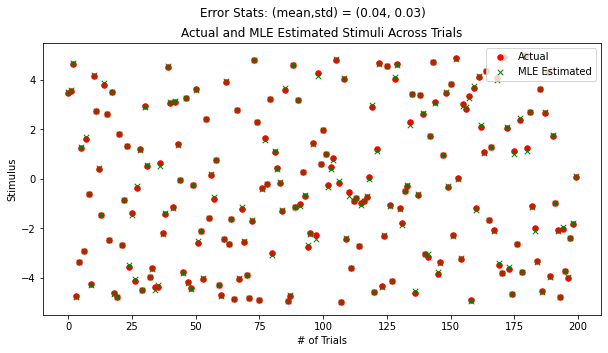
\includegraphics[width = 1\textwidth]{images/Q2/MLE.png}
        \caption{Actual and MLE Estimated Stimuli Across Trials}
    %\label{fig:mesh1}
\end{figure}


Intuitively, from the figure, MLE outperforms the WTA decoder as its shots are more accurate. Let's evaluate the model from its mean absolute error based statistics as follows.


\begin{mintedbox}{python}
print('Error Statistics for MLE Decoder')
print('Mean of errors in stimuli estimation:', error.mean().round(5))
print('Standard deviation of errors in stimuli estimation :', error.std().round(5))
\end{mintedbox}

Error Statistics for MLE Decoder \\
Mean of errors in stimuli estimation: 0.04098\\
Standard deviation of errors in stimuli estimation : 0.03074\\

According to the comparison of error statistics between WTA and MLE decoder, MLE decoder is clear winner as it decreases our error rates more than $\%5$ in average.




\newpage
{\scshape EEE 482} \hfill {\scshape \large  Homework-\romannumeral4\relax} \hfill {\scshape Can Kocagil}
\smallskip
\hrule
\vspace{2mm}


\subsection{Part D}
In this part, we'll make same experiment and simulation as in the part c except for its decoding mechanism. We replace MLE decoder to MAP decoder. MLE and MAP counterparts in the context of probability theory and statistics. MLE treats the unknown variable as unknown constant, and it falls into the classical statistics concept whereas MAP considers unknown variable as random variable with prior distribution and it falls into Bayesian statistics. Hence, in the Bayesian view, they are treated as random variables with known prior. In classical view, they are treated as deterministic quantities that happen to be unknown.

\bigskip
In the settings of the question, we assume that the prior of the stimulus value x follows a Gaussian distribution with a mean of 0 and a standard deviation of 2.5.

\begin{equation*}
   P( x \mid  r_1,...,r_{21}) \underset{\sim}{\propto} P(r_1,...,r_{21}  \mid  x) P(x)
\end{equation*}


\begin{equation*}
   x_{MAP} =  \underset{x}{\mathrm{argmax}} \hspace{1mm} P(r_1,...,r_{21}  \mid  x) P(x) \textit{ where $P(x)$}  \sim \mathcal{N}( \mu = 0, \sigma = 2.5)  
\end{equation*}

We kindly drop the normalization constant in the posterior calculation of $P(x\mid  r_1,...,r_{21})$ since it does not give any further information regarding the estimation of the stimulus except for normalization.

\bigskip
Hence, we can expect that our MAP decoder gives similar analytical expression, but not exactly same. With the MAP decoder settings, we have priory Gaussian denoted by $P(x)$ that affects the analytical derivation. It just adds an extra penalty/regularization term to the analytical expression to the decoder. Since the calculations are very similar to MLE settings except for priory Gaussian aggregation, we directly go to the implementation part as follows.



\begin{mintedbox}{python}
def MAP_decoder(stimuli_interval:np.ndarray = np.linspace(-5,5, 500).tolist(),
                response:np.ndarray = None) -> np.float16:
    """
    Given a population response and  stimuli of the
    neurons, compute the MAP decoder that 
    estimates the actual stimulus as the preferred
    stimulus of the neuron with maximum response

        Arguments:
            stimuli  (np.ndarray): The preferred stimuli of the neurons
            response (np.ndarray): The neural responses
        Returns:
            stimulus (np.float16): the estimated input stimulus that maximizes the response
    """
    logs = list()

    for stim in stimuli_interval:
       
        log = sum((r - gauss_tuning(stim, m)) ** 2 for r, m in zip(response, means))
        log = log * 200 + (stim ** 2) / 10 
        
        logs.append(log)

    idx_stim_max = np.argmin(logs)
    return stimuli_interval[idx_stim_max]
\end{mintedbox}



\newpage
{\scshape EEE 482} \hfill {\scshape \large  Homework-\romannumeral4\relax} \hfill {\scshape Can Kocagil}
\smallskip
\hrule
\vspace{2mm}

We can see that as a additional code to MLE, we simply add the penalty term originated from the priory Gaussian. Let's see the performance of MAP decoder, with its error statistics and prediction visualization.


\begin{mintedbox}{python}
MAP_logs_ = list()
for neural_activity in stimuli_response_:
    response, stimulus = neural_activity[:2]
    estimated_stimulus_MAP = MAP_decoder(stimuli_interval, response)
    MAP_logs_.append((stimulus, estimated_stimulus_MAP, np.abs(stimulus - estimated_stimulus_MAP)))
    
# Tuples are gathered:
MAP_logs = list(zip(*MAP_logs_))

fig = plt.figure(figsize=(10,5))
error = np.array(MAP_logs[2])
fig.suptitle(f'Error Stats: (mean,std) = {round(error.mean(),2),round(error.std(),2)}')
plt.scatter(range(n_trials), MAP_logs[0], marker="o", color="r", s=30, linewidths=1)
plt.scatter(range(n_trials), MAP_logs[1], marker="x", color="green", s=30, linewidths=1)
plt.xlabel('# of Trials')
plt.ylabel('Stimulus')
plt.title('Actual and MAP Estimated Stimuli Across Trials')
plt.legend(['Actual', 'MAP Estimated'], loc='upper right')
plt.show()
\end{mintedbox}


\begin{figure}[h]
    \centering
        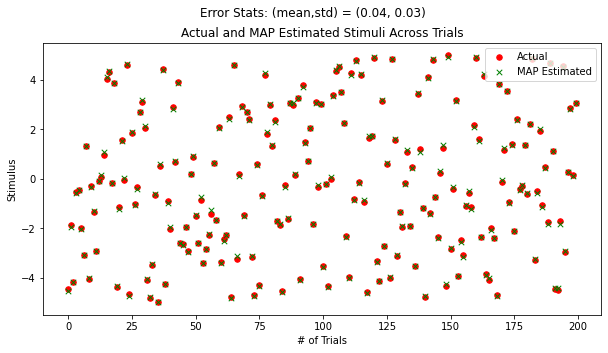
\includegraphics[width = 1\textwidth]{images/Q2/MAP.png}
        \caption{Actual and MAP Estimated Stimuli Across Trials}
    %\label{fig:mesh1}
\end{figure}


\newpage
{\scshape EEE 482} \hfill {\scshape \large  Homework-\romannumeral4\relax} \hfill {\scshape Can Kocagil}
\smallskip
\hrule
\vspace{2mm}

The results are promising. Let's see the error statistics as follows.


\begin{mintedbox}{python}
print('Error Statistics for MAP Decoder')
print('Mean of errors in stimuli estimation:', error.mean().round(5))
print('Standard deviation of errors in stimuli estimation :', error.std().round(5))
\end{mintedbox}

Error Statistics for MAP Decoder \\
Mean of errors in stimuli estimation: 0.04068  \\
Standard deviation of errors in stimuli estimation : 0.0311  \\

As we can compare, the results are very close to the MLE case, MAP outperforms the MLE in averaged error case but it fails to win in error standard deviation comparison. Hence, the variance of MAP predictions have less bias then MLE case, but it has higher variance than MLE.


\subsection{Part E}
In this part, we'll perform an experiment with 200 trials of stimulus intensity. In each trial, sample a stimulus intensity from the interval $[-5, 5]$. For the resulting stimulus vector (of length 200),
we'll separately simulate the population response vectors r for $\sigma_i$ = 0.1, $\sigma_i$ = 0.2, $\sigma_i$ = 0.5, $\sigma_i$ = 1, $\sigma_i$ = 2, and $\sigma_i$ = 5. In each case, we assume additive Gaussian noise with zero mean and $1/20$ standard deviation. After that, we'll calculate MLE estimates of the stimulus $x_{ML}$ based on each population response separately. 

\bigskip
Since this question is direct computational problem, let's quickly dive into code as follows.


\begin{mintedbox}{python}
stds = [0.1, 0.2, 0.5, 1.0, 2.0, 5.0]
bias_outer = []

for stimuli in random.sample(stimuli_interval.tolist(), n_trials):
    bias_inner = []
    for std in stds:
        response = gauss_tuning(stimuli,means,sigma=std)
        response += np.random.normal(loc = 0, scale = 1/20, size = (21,)) 
        stimulus_MLE = MLE_decoder(response=response)
        bias = np.abs(stimuli - stimulus_MLE)
        bias_inner.append(bias)
    bias_outer.append(tuple(bias_inner))
 # Tuples are gathered:
sigmas_response_bias = list(zip(*bias_outer)) 
\end{mintedbox}

Then, let's see the error results with table format as follows.

\begin{mintedbox}{python}
error_stats = {}
for bias, sigma in zip(sigmas_responses,stds):
    ave_error = np.mean(bias).round(3)
    std_error = np.std(bias).round(3)
    error_stats[sigma] = ave_error, std_error
error_stats = pd.DataFrame(error_stats).T
error_stats.columns = ['Mean Error','STD Error']
error_stats.index = stds
error_stats.index.name = 'Sigma Values'
error_stats.sort_values('Mean Error', ascending = True,inplace = True)
error_stats.head(n = 6) 
\end{mintedbox}


Here is the table representation of error statistics.



% Please add the following required packages to your document preamble:
% 
\begin{table*}[]
\begin{tabular}{@{}lll@{}}
\toprule
             & \textbf{Mean Error} & \textbf{STD Error} \\ \midrule
\textbf{Sigma Values} &                     &                    \\
1.0          & 0.044               & 0.032              \\
0.5          & 0.055               & 0.039              \\
2.0          & 0.092               & 0.062              \\
5.0          & 0.371               & 0.280              \\
0.2          & 0.515               & 1.313              \\
0.1          & 1.877               & 2.371              \\ \bottomrule
\end{tabular}
\caption{\label{tab:table-name}Error Statistics based on $\sigma$ values with MLE}
\end{table*}

\newpage
We can see that we have optimal $\sigma$ value at $\sigma$ = 1.0. Moreover, there is no linear pattern that $\sigma$ values reasons to error. Let's see the distribution of $\sigma$ values on mean and standard deviation of errors.

\begin{mintedbox}{python}
fig, ax = plt.subplots(figsize = (10,5))
error_stats.plot.kde(ax=ax)
error_stats.plot.hist(density=True, ax = ax)
ax.set_ylabel('Error Stats')
ax.set_xlabel('Sigma values $\sigma$')
ax.grid()

fig, ax = plt.subplots(figsize = (10,5))
error_stats.plot(ax=ax,marker = 'o')
ax.set_ylabel('Error Stats')
ax.set_xlabel('Sigma values $\sigma$')
ax.grid()
\end{mintedbox}

\begin{figure}[h]
    \centering
        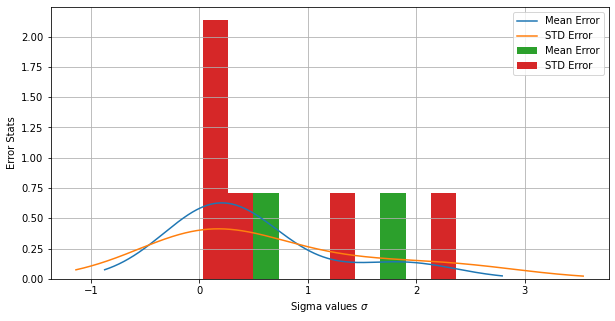
\includegraphics[width = 1\textwidth]{images/Q2/hist.png}
        \caption{Histogram and Density Plot of Error Rate w.r.t. varying $\sigma$}
    %\label{fig:mesh1}
\end{figure}

\newpage
{\scshape EEE 482} \hfill {\scshape \large  Homework-\romannumeral4\relax} \hfill {\scshape Can Kocagil}
\smallskip
\hrule
\vspace{2mm}


\begin{figure}[h]
    \centering
        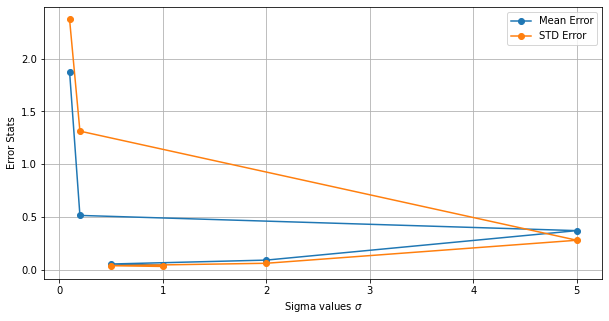
\includegraphics[width = 1\textwidth]{images/Q2/plot.png}
        \caption{Plot of Error Rate w.r.t. varying $\sigma$}
    %\label{fig:mesh1}
\end{figure}

From the figures, we can conclude that there is no linear pattern of error rates w.r.t. varying parameter $\sigma$. But, we can see that we have optimal $\sigma$ value at $\sigma$ = 1.0 that minimizes the error rates based on MLE decoder. Since there is no direct correlation between the narrowness of the Gaussian and error rates, one cannot generalize the effects of $\sigma$ of the Gaussian tuning with error rates based on the MLE decoder.
\newpage


\newpage
{\scshape EEE 482} \hfill {\scshape \large  Homework-\romannumeral4\relax} \hfill {\scshape Can Kocagil}
\smallskip
\hrule
\vspace{2mm}

\section{Source Code}

\begin{mintedbox}{python}
#!/usr/bin/env python
# coding: utf-8
# In[4]:


# Imports:
import numpy as np, matplotlib.pyplot as plt, scipy.stats as stats, pandas as pd
from sklearn.decomposition import PCA, FastICA, NMF
import random, h5py

settings = np.seterr(all='ignore')


# ### Part A

# In[5]:


# Retrieving data:
faces = h5py.File('hw4_data1.mat','r')['faces'][:].T

print(faces.shape)


# In[6]:


# Little bit of dimension manipulation for representing images:
N, num_pixel = faces.shape
image_faces = faces.reshape(N, np.int(np.sqrt(num_pixel)), np.int(np.sqrt(num_pixel)))
print(image_faces.shape)


# In[7]:


# Let's look at the face images:
fig, axs = plt.subplots(3,3,figsize = (8,8))
for i, axes in enumerate(axs.flatten()):
    axes.imshow(image_faces[i], cmap = 'gray')
    axes.axis('off')


# In[8]:


# Latent representation dimension:
latent_dim = 100
pca = PCA(n_components = latent_dim)
principalComponents = pca.fit_transform(faces)

num2str = lambda x : str(round(sum(x),3))

legends = [

    pca.explained_variance_ratio_[:10],
    pca.explained_variance_ratio_[:25],
    pca.explained_variance_ratio_[:50],
    pca.explained_variance_ratio_[:]

]

legends = list(map(num2str,legends))

plt.figure(figsize = (10,5))
plt.plot(pca.explained_variance_ratio_, color = 'r')
plt.xlabel('PCs')
plt.ylabel('Explained Variance')
title = 'Principal Components versus Explained Variance \n'
title += 'First (10,25,50,100) PCs explained variance = '
title += '('  + ' '.join(legends) + ')'
plt.title(title)
plt.grid()
plt.show()


pca_logs = f'Variance explained by PCA for 10 components  {legends[0]} \n'
pca_logs += f'Variance explained by PCA for 25 components  {legends[1]} \n'
pca_logs += f'Variance explained by PCA for 50 components  {legends[2]} \n'
pca_logs += f'Variance explained by PCA for 100 components {legends[3]}'
print(pca_logs)


# In[9]:


fig, axes = plt.subplots(5, 5, figsize=(12,12))
for i, ax in enumerate(axes.flat):
    ax.imshow(pca.components_[i].reshape(32, 32).T, cmap = 'gray')
    ax.axis('off')


# ### Part B

# In[10]:


def pca_reconstruction(data:np.ndarray,
                       trained_pca:PCA,
                       number_PCs:int) -> np.ndarray:
    """
    
        Given the input data, trained PCA variable and # of PCs, reconstruct images based on the PCs components.
        
            
        Arguments:
            - data (np.ndarray) : Input data
            - trained_pca (PCA) : trained PCA variable
            - number_PCs (int)  : # of PCs to reconstruct images
            
        Returns:
            - reconstructed_data (np.ndarray) : Reconsturcted/Predicted data via given # of PCs
    
    
    """
    
    pca_mean = trained_pca.mean_ 
    mean_removed = data - pca_mean
    pca_components = trained_pca.components_[:number_PCs]
    
    return mean_removed @ pca_components.T @ pca_components + pca_mean


def plot_faces(faces:np.ndarray,
               suptitle:str) -> None:
    """
        
        Given the face and its suptitle, plots the 6x6 grid.
        
        Arguments:
            - faces       (np.ndarray) : Face data to be plotted
            - suptitle    (str)        : Suptitle of the visualizatiom
            
        Returns:
            - None

    """
    
    fig, axes = plt.subplots(6, 6, 
                             figsize=(10,10),
                             facecolor='white',
                             subplot_kw= {
                                 'xticks': [],
                                 'yticks':[]
                             }
    )
    fig.suptitle(suptitle,
                 fontsize = '14')
                 
    fig.tight_layout(rect = [0, 0, 1, .95])
    
    for i, ax in enumerate(axes.flat):
        ax.imshow(faces[i].reshape(32, 32).T, cmap='gray')
        ax.set_xlabel(i+1)


# In[11]:


faces_PCA_10 = pca_reconstruction(faces,pca,10)
faces_PCA_25 = pca_reconstruction(faces,pca,25)
faces_PCA_50 = pca_reconstruction(faces,pca,50)
faces_PCA_100 = pca.inverse_transform(principalComponents)


# In[12]:


plot_faces(faces,suptitle = 'Original Versions of the First 36 Images')


# In[13]:


plot_faces(faces_PCA_10,suptitle = 'Reconstructed 36 images based on first 10 PCs')


# In[14]:


plot_faces(faces_PCA_25,suptitle = 'Reconstructed 36 images based on first 25 PCs')


# In[15]:


plot_faces(faces_PCA_50,suptitle = 'Reconstructed 36 images based on first 50 PCs')


# In[16]:


plot_faces(faces_PCA_100, suptitle = 'Reconstructed 36 images based on first 100 PCs')


# In[17]:


def squared_error(y_true:np.ndarray,y_pred:np.ndarray) -> np.ndarray:
    """
        Given the grounth truth matrix and prediction, computes element wise squared error.
        
            
        Arguments:
            - y_true  (np.ndarray) : grounth truth
            - y_pred  (np.ndarray) : prediction
            
        Returns:
            square_error (np.ndarray) : Point-wise MSE loss
    
    """
    assert y_true.shape == y_pred.shape, f'Mismatch Dimension!, {y_true.shape} does not match with {y_pred.shape}'
    return (y_true - y_pred) ** 2


# In[18]:


mse_10 = squared_error(y_true = faces, y_pred = faces_PCA_10)
mse_25 = squared_error(y_true = faces, y_pred = faces_PCA_25)
mse_50 = squared_error(y_true = faces, y_pred = faces_PCA_50)


std_mse_10 = mse_10.mean(-1).std()
std_mse_25 = mse_25.mean(-1).std()
std_mse_50 = mse_50.mean(-1).std()

mean_mse_10 = mse_10.mean()
mean_mse_25 = mse_25.mean()
mean_mse_50 = mse_50.mean()


print(f'PCA reconstruction loss stats based on first 10 PCs, \n (mean,std) = {mean_mse_10,std_mse_10}')
print(f'PCA reconstruction loss stats based on first 25 PCs, \n (mean,std) = {mean_mse_25,std_mse_25}')
print(f'PCA reconstruction loss stats based on first 50 PCs, \n (mean,std) = {mean_mse_50,std_mse_50}')


# ### Part C

# In[19]:


fastIca_10 = FastICA(n_components = 10, random_state = 5)
fastIca_components_10 = fastIca_10.fit_transform(faces)


fig, axes = plt.subplots(2, 5, figsize=(10,4))
for i, ax in enumerate(axes.flat):
    ax.imshow(fastIca_10.components_[i].reshape(32, 32).T, cmap = 'gray')
    ax.axis('off')


# In[20]:


fastIca_25 = FastICA(n_components = 25,whiten = True, random_state = 5)
fastIca_components_25 = fastIca_25.fit_transform(faces)


fig, axes = plt.subplots(5, 5, figsize=(10,10))
for i, ax in enumerate(axes.flat):
    ax.imshow(fastIca_25.components_[i].reshape(32, 32).T, cmap = 'gray')
    ax.axis('off')


# In[21]:


fastIca_50 = FastICA(n_components = 50, random_state = 5)
fastIca_components_50 = fastIca_50.fit_transform(faces)


fig, axes = plt.subplots(5, 10, figsize=(20,10))
for i, ax in enumerate(axes.flat):
    ax.imshow(fastIca_50.components_[i].reshape(32, 32).T, cmap = 'gray')
    ax.axis('off')


# In[22]:


faces_ICA_10 = fastIca_10.inverse_transform(fastIca_components_10)
faces_ICA_25 = fastIca_25.inverse_transform(fastIca_components_25)
faces_ICA_50 = fastIca_50.inverse_transform(fastIca_components_50)


# In[23]:


plot_faces(faces_ICA_10, suptitle = 'FastICA reconstruction based on 10 independent components')


# In[24]:


plot_faces(faces_ICA_25, suptitle = 'FastICA reconstruction based on 25 independent components')


# In[25]:


plot_faces(faces_ICA_50, suptitle = 'FastICA reconstruction based on 50 independent components')


# In[26]:


mse_10 = squared_error(y_true = faces, y_pred = faces_ICA_10)
mse_25 = squared_error(y_true = faces, y_pred = faces_ICA_25)
mse_50 = squared_error(y_true = faces, y_pred = faces_ICA_50)


std_mse_10 = mse_10.mean(-1).std()
std_mse_25 = mse_25.mean(-1).std()
std_mse_50 = mse_50.mean(-1).std()

mean_mse_10 = mse_10.mean()
mean_mse_25 = mse_25.mean()
mean_mse_50 = mse_50.mean()


print(f'ICA reconstruction loss stats based on first 10 ICs, \n (mean,std) = {mean_mse_10,std_mse_10}')
print(f'ICA reconstruction loss stats based on first 25 ICs, \n (mean,std) = {mean_mse_25,std_mse_25}')
print(f'ICA reconstruction loss stats based on first 50 ICs, \n (mean,std) = {mean_mse_50,std_mse_50}')


# In[27]:


"""
fastICA can be seen as whitening (which can be achieved by PCA) plus an orthogonal rotation (an orthogonal rotation such that the estimated sources are as non-gaussian as possible).

The orthogonal rotation does not affect the reconstruction error of the ICA solution and hence you have the same reconstruction error for PCA and ICA.

"""


# In[28]:


from sklearn.preprocessing import MinMaxScaler


# ### Part D

# In[29]:


faces = h5py.File('hw4_data1.mat','r')['faces'][:].T
max_iter = 500
faces += np.abs(np.min(faces))
NMF_10 = NMF(n_components = 10, max_iter = max_iter)
NMF_components_10 = NMF_10.fit_transform(faces)


fig, axes = plt.subplots(2, 5, figsize=(10,4))
for i, ax in enumerate(axes.flat):
    ax.imshow(NMF_10.components_[i].reshape(32, 32).T, cmap = 'gray')
    ax.axis('off')


# In[30]:


NMF_25 = NMF(n_components = 25, max_iter = max_iter)
NMF_components_25 = NMF_25.fit_transform(faces)


fig, axes = plt.subplots(5, 5, figsize=(10,10))
for i, ax in enumerate(axes.flat):
    ax.imshow(NMF_25.components_[i].reshape(32, 32).T, cmap = 'gray')
    ax.axis('off')


# In[31]:


NMF_50 = NMF(n_components = 50, max_iter = max_iter)
NMF_components_50 = NMF_50.fit_transform(faces)


fig, axes = plt.subplots(5, 10, figsize=(12,6))
for i, ax in enumerate(axes.flat):
    ax.imshow(NMF_50.components_[i].reshape(32, 32).T, cmap = 'gray')
    ax.axis('off')


# In[32]:


faces = h5py.File('hw4_data1.mat','r')['faces'][:].T

faces_NNMF_10 = NMF_10.inverse_transform(NMF_components_10) - np.abs(np.min(faces))
faces_NNMF_25 = NMF_25.inverse_transform(NMF_components_25) - np.abs(np.min(faces))
faces_NNMF_50 = NMF_50.inverse_transform(NMF_components_50) - np.abs(np.min(faces))


# In[ ]:





# In[33]:


plot_faces(faces_NNMF_10, suptitle = 'NNMF Reconstruction of faces based on 10MFs')


# In[34]:


plot_faces(faces_NNMF_25, suptitle = 'NNMF Reconstruction of faces based on 25MFs')


# In[35]:


plot_faces(faces_NNMF_50, suptitle = 'NNMF Reconstruction of faces based on 50MFs')


# In[36]:


mse_10 = squared_error(y_true = faces, y_pred = faces_NNMF_10)
mse_25 = squared_error(y_true = faces, y_pred = faces_NNMF_25)
mse_50 = squared_error(y_true = faces, y_pred = faces_NNMF_50)


std_mse_10 = mse_10.mean(-1).std()
std_mse_25 = mse_25.mean(-1).std()
std_mse_50 = mse_50.mean(-1).std()

mean_mse_10 = mse_10.mean()
mean_mse_25 = mse_25.mean()
mean_mse_50 = mse_50.mean()


print(f'NNMF reconstruction loss stats based on first 10 MFs, \n (mean,std) = {mean_mse_10,std_mse_10}')
print(f'NNMF reconstruction loss stats based on first 25 MFs, \n (mean,std) = {mean_mse_25,std_mse_25}')
print(f'NNMF reconstruction loss stats based on first 50 MFs, \n (mean,std) = {mean_mse_50,std_mse_50}')


# #### Q2

# ### Part A

# In[38]:


def gauss_tuning(x:np.ndarray = np.linspace(-15, 16, 500),
                 mu:float = 1,
                 sigma:float = 1,
                 A:float = 1) -> np.float16:
    """
        Gaussian shaped tuning function of a population of neurons.

        Arguments:
            x     (np.ndarray)   : The input stimulus parameters
            A     (float)        : Gain of the Gaussian-shaped tuning curve
            mu    (float)   : Mean of the Gausssian-shaped tuning curve
            sigma (float)        : Standard deviation of the Gaussian-shaped tuning curve

        Returns:
            response : Resulting neural response
        """             
    return A * np.exp(-0.5 * ((x- mu)/sigma) ** 2)


# In[39]:


neural_responses = []
legends = []
stimuli = np.linspace(-15, 16, 500)
means = np.arange(-10, 11)
plt.figure(figsize=(10,5))

for mean in means:
    response = gauss_tuning(mu = mean)
    plt.plot(stimuli, response)
    legends.append(f" Response with mean {mean}")
    
    # Let's keep neural responses for future use:
    neural_responses.append(response)

# Plot the tuning profiles
plt.plot(stimuli, np.mean(neural_responses, axis=0), color = '0')
legends.append(f" Average Response")
plt.legend(legends, loc="right", bbox_to_anchor=(1.4, 0.5))
plt.xlabel('Stimulus')
plt.ylabel('Activity')
plt.title('Tuning Curves of a Population of Neurons')
plt.grid()
plt.show()


# In[40]:


kwargs = dict(
            color = '0',
            marker= 'o',
            markerfacecolor='red'
)
plt.figure(figsize=(10,5))
plt.plot(means, gauss_tuning(-1, mu = means),**kwargs)
plt.xlabel('Preferred Stimulus')
plt.ylabel('Population Response')
plt.title('Population Response to the Stimulus x = -1 vs Preferred Stimuli of Neurons')
plt.grid()
plt.show()


# ### Part B

# 

# In[51]:


def WTA_decoder(stimuli:np.ndarray,response:np.ndarray) -> np.float16:
    """
    Given a population response and  stimuli of the
    neurons, compute the winner-take-all decoder that 
    estimates the actual stimulus as the preferred
    stimulus of the neuron with maximum response

        Arguments:
            stimuli  (np.ndarray): The preferred stimuli of the neurons
            response (np.ndarray): The neural responses
        Returns:
            stimulus (np.float16): the estimated input stimulus that maximizes the response
    """

    response += np.random.normal(loc = 0, scale = 1/20, size = (21,)) 
    return stimuli[np.argmax(response)]


# In[52]:


n_trials = 200
stimuli_interval = np.linspace(-5,5, 500).tolist()

# To keep 'responses','stimuli','WTA_stimuli','Errors'
stimuli_response_ = []

for stimuli in random.sample(stimuli_interval, n_trials):
    response = gauss_tuning(stimuli, mu = means)
    WTA_stimuli = WTA_decoder(means, response)
    stimuli_response_.append((response, stimuli, WTA_stimuli, np.abs(WTA_stimuli - stimuli)))
 
# Tuples are gathered:
stimuli_response = list(zip(*stimuli_response_))


# In[53]:


fig = plt.figure(figsize=(10,5))
error = np.array(stimuli_response[-1])
fig.suptitle(f'Error Stats: (mean,std) = {round(error.mean(),2),round(error.std(),2)}')
plt.scatter(range(n_trials), stimuli_response[1], marker="o", color="r", s=30, linewidths=1)
plt.scatter(range(n_trials), stimuli_response[2], marker="x", color="green", s=30, linewidths=1)
plt.xlabel('# of Trials')
plt.ylabel('Stimulus')
plt.title('Actual and WTA Estimated Stimuli Across Trials')
plt.legend(['Actual', 'WTA Estimated'], loc='upper right')
plt.show()


# In[57]:


print('Error Statistics for Winner Take All Decoder')
print('Mean of errors in stimuli estimation:', error.mean().round(5))
print('Standard deviation of errors in stimuli estimation :', error.std().round(5))


# ### Part C

# In[45]:


def MLE_decoder(stimuli_interval:np.ndarray = np.linspace(-5,5, 500).tolist(),
                response:np.ndarray = None) -> np.float16:
     
    """
    Given a population response and  stimuli of the
    neurons, compute the MLE decoder that 
    estimates the actual stimulus as the preferred
    stimulus of the neuron with maximum response

        Arguments:
            stimuli  (np.ndarray): The preferred stimuli of the neurons
            response (np.ndarray): The neural responses
        Returns:
            stimulus (np.float16): the estimated input stimulus that maximizes the response
    """


    logs = list()

    for stim in stimuli_interval:
        log = sum((response_ - gauss_tuning(stim, mu_)) ** 2 for response_, mu_ in zip(response, means)) 
           
        logs.append(log)

    idx_stim_max = np.argmin(logs)
    return stimuli_interval[idx_stim_max]
        


# In[59]:


MLE_logs_ = list()
for neural_activity in stimuli_response_:
    response, stimulus = neural_activity[:2]
    estimated_stimulus_MLE = MLE_decoder(stimuli_interval, response)
    MLE_logs_.append((stimulus, estimated_stimulus_MLE, np.abs(stimulus - estimated_stimulus_MLE)))
    
            
# Tuples are gathered:
MLE_logs = list(zip(*MLE_logs_))


# In[60]:


fig = plt.figure(figsize=(10,5))
error = np.array(MLE_logs[2])
fig.suptitle(f'Error Stats: (mean,std) = {round(error.mean(),2),round(error.std(),2)}')
plt.scatter(range(n_trials), MLE_logs[0], marker="o", color="r", s=30, linewidths=1)
plt.scatter(range(n_trials), MLE_logs[1], marker="x", color="green", s=30, linewidths=1)
plt.xlabel('# of Trials')
plt.ylabel('Stimulus')
plt.title('Actual and MLE Estimated Stimuli Across Trials')
plt.legend(['Actual', 'MLE Estimated'], loc='upper right')
plt.show()


# In[61]:


print('Error Statistics for MLE Decoder')
print('Mean of errors in stimuli estimation:', error.mean().round(5))
print('Standard deviation of errors in stimuli estimation :', error.std().round(5))


# In[ ]:





# ### Part D

# In[62]:


def MAP_decoder(stimuli_interval:np.ndarray = np.linspace(-5,5, 500).tolist(),
                response:np.ndarray = None) -> np.float16:
     
    """
    Given a population response and  stimuli of the
    neurons, compute the MAP decoder that 
    estimates the actual stimulus as the preferred
    stimulus of the neuron with maximum response

        Arguments:
            stimuli  (np.ndarray): The preferred stimuli of the neurons
            response (np.ndarray): The neural responses
        Returns:
            stimulus (np.float16): the estimated input stimulus that maximizes the response
    """


    logs = list()

    for stim in stimuli_interval:

       
        log = sum((r - gauss_tuning(stim, m)) ** 2 for r, m in zip(response, means))
        log = log * 200 + (stim ** 2) / 10 
        
        logs.append(log)

    idx_stim_max = np.argmin(logs)
    return stimuli_interval[idx_stim_max]
        


# In[63]:


MAP_logs_ = list()
for neural_activity in stimuli_response_:
    response, stimulus = neural_activity[:2]
    estimated_stimulus_MAP = MAP_decoder(stimuli_interval, response)
    MAP_logs_.append((stimulus, estimated_stimulus_MAP, np.abs(stimulus - estimated_stimulus_MAP)))
    
            
# Tuples are gathered:
MAP_logs = list(zip(*MAP_logs_))


# In[64]:


fig = plt.figure(figsize=(10,5))
error = np.array(MAP_logs[2])
fig.suptitle(f'Error Stats: (mean,std) = {round(error.mean(),2),round(error.std(),2)}')
plt.scatter(range(n_trials), MAP_logs[0], marker="o", color="r", s=30, linewidths=1)
plt.scatter(range(n_trials), MAP_logs[1], marker="x", color="green", s=30, linewidths=1)
plt.xlabel('# of Trials')
plt.ylabel('Stimulus')
plt.title('Actual and MAP Estimated Stimuli Across Trials')
plt.legend(['Actual', 'MAP Estimated'], loc='upper right')
plt.show()


# In[66]:


print('Error Statistics for MAP Decoder')
print('Mean of errors in stimuli estimation:', error.mean().round(5))
print('Standard deviation of errors in stimuli estimation :', error.std().round(5))


# ### Part E

# In[144]:


stds = [0.1, 0.2, 0.5, 1.0, 2.0, 5.0]
bias_outer = []

for stimuli in random.sample(stimuli_interval.tolist(), n_trials):
    bias_inner = []
    for std in stds:
        response = gauss_tuning(stimuli,means,sigma=std)
        response += np.random.normal(loc = 0, scale = 1/20, size = (21,)) 
        stimulus_MLE = MLE_decoder(response=response)
        bias = np.abs(stimuli - stimulus_MLE)
        bias_inner.append(bias)

    bias_outer.append(tuple(bias_inner))

 # Tuples are gathered:
sigmas_response_bias = list(zip(*bias_outer))   


# In[227]:


error_stats = {}

for bias, sigma in zip(sigmas_responses,stds):
  
    ave_error = np.mean(bias).round(3)
    std_error = np.std(bias).round(3)
    error_stats[sigma] = ave_error, std_error
        
error_stats = pd.DataFrame(error_stats).T
error_stats.columns = ['Mean Error','STD Error']
error_stats.index = stds
error_stats.index.name = 'Sigma Values'
error_stats.sort_values('Mean Error', ascending = True,inplace = True)
error_stats.head(n = 6)


# 

# In[230]:


fig, ax = plt.subplots(figsize = (10,5))
error_stats.plot.kde(ax=ax)
error_stats.plot.hist(density=True, ax = ax)
ax.set_ylabel('Error Stats')
ax.set_xlabel('Sigma values $\sigma$')
ax.grid()


fig, ax = plt.subplots(figsize = (10,5))
error_stats.plot(ax=ax,marker = 'o')
ax.set_ylabel('Error Stats')
ax.set_xlabel('Sigma values $\sigma$')
ax.grid()



# In[ ]:





\end{mintedbox}


\newpage
{\scshape EEE 482} \hfill {\scshape \large  Homework-\romannumeral4\relax} \hfill {\scshape Can Kocagil}
\smallskip
\hrule
\vspace{2mm}

\printbibliography


\end{document}